\documentclass[a4paper, 12pt]{report}
\usepackage{graphicx} % Required for inserting images
\usepackage[T1]{fontenc}
\usepackage[latin1]{inputenc}
\usepackage{glossaries}
\usepackage{graphicx}
\usepackage{amsfonts}
\usepackage{pifont}
\usepackage{eufrak}
\usepackage{amssymb}
\usepackage{listings}
\usepackage{verbatim}
\usepackage{tikz}
\usetikzlibrary{shapes,arrows}
\usepackage{tikz}
\tikzstyle{mybox} = [draw=black, thin, rectangle, rounded corners, inner ysep=5pt, inner xsep=5pt, fill=blue!15]
\newtheorem{theorem}{Teorema}
\usepackage[a4paper, top=2cm , bottom=2cm , right=2cm , left=2cm ]{geometry}

\title{
    {\color{red}
    \textbf{  \Huge{  NON LINEAR CONTROL AND\\ 
    AEROSPACE APPLICATIONS } }\\}
    \textit{Lecture notes}
    \linespread{2}
}
\author{Carlo Migliaccio}
\date{AA 2023/2024}

\begin{document}

%----------------------descrizione blocchi--------------------

\maketitle
\tableofcontents

\part{Non linear modeling and control}
\chapter{Introduction}  
\section{Dynamic Systems, Variables, Signals}
A \textbf{Dynamic System}, roughly speaking, is a collection of interacting object which evolve over the time. Some examples could be: vehicles, mechanical systems, spacecrafts etc.\\
The \textit{time evolution} of these systems can be described by quantities called \textbf{variables}. The functions which describe the evolution over the time of such quantities play an important role and they are called \textbf{signals}.\\
Among all variables there are some of them which are particularly important such as: 
\begin{itemize}
\setlength\itemsep{0em}
    \item \textbf{Input} $u(t)$: variables that influence the time evolution of the system, the so called causes. We can distinguish two types of input: 
    \begin{enumerate}
        \item \textbf{Command input}: a human user can choose it;
        \item \textbf{Disturbance}: as their presence is not under the control of a human, they can't be chosen.
    \end{enumerate}
    \item \textbf{Causes} $y(t)$: measured variables;
\end{itemize}

\tikzstyle{block} = [draw, fill=white, rectangle, minimum height=3em, minimum width=6em]
\tikzstyle{sum} = [draw, fill=white, circle, node distance=1cm]
\tikzstyle{input} = [coordinate]
\tikzstyle{output} = [coordinate]
\tikzstyle{pinstyle} = [pin edge={to-,thin,black}]

%-----------------diagramma a blocchi d'esempio--------------------------
\begin{comment}
\begin{tikzpicture}[auto, node distance=2cm,>=latex']
    \node [input, name=input] {};
    \node [sum, right of=input] (sum) {};
    \node [block, right of=sum] (controller) {Controller};
    \node [block, right of=controller, pin={[pinstyle]above:D},
            node distance=3cm] (system) {System};

    \draw [->] (controller) -- node[name=u] {$u$} (system);
    \node [output, right of=system] (output) {};
    \node [block, below of=u] (measurements) {Measurements};

    \draw [draw,->] (input) -- node {$r$} (sum);
    \draw [->] (sum) -- node {$e$} (controller);
    \draw [->] (system) -- node [name=y] {$y$}(output);
    \draw [->] (y) |- (measurements);
    \draw [->] (measurements) -| node[pos=0.99] {$-$} 
        node [near end] {$y_m$} (sum);
\end{tikzpicture}
\end{comment}

\begin{figure}
    \centering

    \begin{tikzpicture}[auto, node distance=2cm,>=latex']
        \node[input, name=input] {}; 
        \node[block, right of=input] (system) {System};
        \node[output, right  of=system, name=output]{}; 

        \draw[->](system) -- node[name=u]{$u(t)$}(input);
        \draw[->] (system) -- node[name=y]{$y(t)$}(output);
    \end{tikzpicture}

    
    \caption{Rappresentazione a blocchi di un sistema dinamico}
    \label{fig:enter-label}
\end{figure}

%-------------------------------------------------------------
\section{General considerations}
In the area of automatic control and dynamic systems, is important to distinguish between:
\begin{itemize}
    \item \textbf{Physical system} (which we call the \textbf{plant});
    \item The \textbf{model}: can be defined as a mathematical description of the variables.
\end{itemize}
A model is important for several reasons: to make a prediction, filtering, analyze a system, control it... Despite these important aspects, we ought to remember that \textit{models represent an approximation of the real system}. For this reason we have to deal with uncertainty of two types: 
\begin{enumerate}
\setlength\itemsep{0em}
    \item \textbf{Parametric}: caused by approximation of the parameters; 
    \item \textbf{Dynamic}: caused by the fact of overall some details in the description of the model which rarely is exactly known and so easily descripted. 
\end{enumerate}

To deal efficiently with \textit{uncertainty} we need \textbf{robust} techniques for modeling and control such types of systems.

%----------------------------------------------------------
\section {State equations}
A \textbf{dynamic system} can be always described by a \textbf{set of first order differential equations}:

    \begin{align}    
        &\dot{x}=f[x(t), u(t), t]\\
        &y(t)=h[x(t), u(t), t]
    \end{align}

where: 
\begin{itemize}
    \setlength\itemsep{0em}
    \item $x(t)\in\mathbb{R}^{n_x}$ is the \textbf{state}; 
    \item $u(t) \in\mathbb{R}^{n_u}$ is the \textbf{input}; 
    \item $y(t) \in\mathbb{R}^{n_y}$ is the \textbf{output}; 
    \item $n_x$ is the \textbf{order of the system}, is important because it tells us how many variables we need to describe the system.
\end{itemize}

This description is standard and sufficiently \textbf{general} to represent any dynamical system. Moreover it is used by many \textit{control design method}.

\subsubsection*{Interpretation of the state equation}
Since the state equation $$\dot{x}=f[x(t),u(t),t]$$ is \textbf{dynamic} and it can be written in local form as $$x(t+dt)=x(t)+f[x,u,t]dt$$ it is clear that locally it can have the following meaning: the state in a time $t+dt$ is equal to the current state $x(t)$ to which we add a variation $fdt$.\\
Differently the \textbf{output equation} is \textbf{static} in the sense that it represents a relation between variables at the same time $t$.\\
In order to concluding this discussion we say that in general the functions $f$ and $g$ are \textit{vector field}.

\section{Classifications of dynamical systems}
According to the characteristic we observe of a dynamic system there could be several classifications. We can mention the most important: 
\begin{itemize}
    \item \textbf{Non Linear systems}: here the functions $f(x,u,t)$ and $h(x,u,t)$ are not linear, the great majority of the systems in nature \textbf{are non linear!}
    \item \textbf{Linear systems}: here we can write the equations previosly seen in the form: 
    \begin{align*}
        &\dot{x}(t) =A(t)x(t)+B(t)u(t)\\
        &y(t)=C(t)x(t)+D(t)u(t)
    \end{align*}
    here \textit{f, h} are linear while the matrices $A(t), B(t), C(t), D(t)$ are possibly time varying; if they are constant we identify a particular (very important) case which is the Linear Time Invariant system (\textbf{LTI}); 
    \item \textbf{Time varying (Time Invariant) systems} here we have: 
    \begin{align*}
        \frac{\partial f}{\partial t}\ne0     \quad   &\frac{\partial g}{\partial t}\ne 0\\
        (\frac{\partial f}{\partial t}= 0     \quad   &\frac{\partial g}{\partial t}= 0)
    \end{align*}
    The functions $f, h$ (do not) explicitly depend on the time; 
    \item  \textbf{Continuous time/Discrete Time} in the former case we have that the variable $t$ is a real positive number, that is $t\in\mathbb{R}^+$, in the latter case we have that the variable $t$ (also indicated with $k$) is a natural number, that is $t\in \mathbb{N}$;
    \item The last classification is based on the \textbf{number of inputs and outputs} ($n_y, n_u$). Specifically we have:
    \begin{enumerate}
        \item \textbf{SISO} (Single input, Single output) $\rightarrow n_u=1, n_y=1$
        \item \textbf{MIMO} (Multiple input, Multiple output) $\rightarrow n_u>1, n_y>1$
        \item \textbf{SIMO} (Single input, Multiple Output)$\rightarrow n_u=1, n_y>1$ 
        \item \textbf{MISO} (Multiple input, single Output)$\rightarrow n_u>1, n_y=1$ 
    \end{enumerate}
    
\end{itemize}


\chapter{Stability concepts}

\textbf{Stabilty} is a very important notion we would like analyzing of a system in order to study his behaviour over the time.


\section{Some definitions}
Let us  consider the system $\mathcal{S}$ which has state equation equal to $$\dot{x(t)}=f[x(t), u(t),t]$$ with input signal $u(t)$ and \textbf{initial conditions} $x(0)$.\\

\noindent
\textbf{Definition} \textit{(Solution of a system)} The signal resulting from the system integration is a \textbf{function of the time} $x(t), \quad  t\ge0$ which is called the \textbf{solution} of the system {\color{blue}\textbf{corresponding to} the initial state $x(0)$ and the input $u(t)$}.\\

\noindent
\textbf{Definition} \textit{(Trajectory of a system)} The \textbf{set of the points of the state space generated by the solution} is called a \textbf{trajectory of the system} corresponding to the initial state $x(0)$ and the input $u(t)$. \\

\noindent
Let $x(t)$ be the \textit{solution} of the system with the respecto to the couple  (initial condition, input) equal to ($x(0), u(t)$), we call it the \textbf{nominal solution}. If we change a bit the initial state to $x^p(t)\ne x(t)$ but with the same input signal we have the \textbf{perturbed solution}.\\

\begin{figure*}[h]
    \centering
    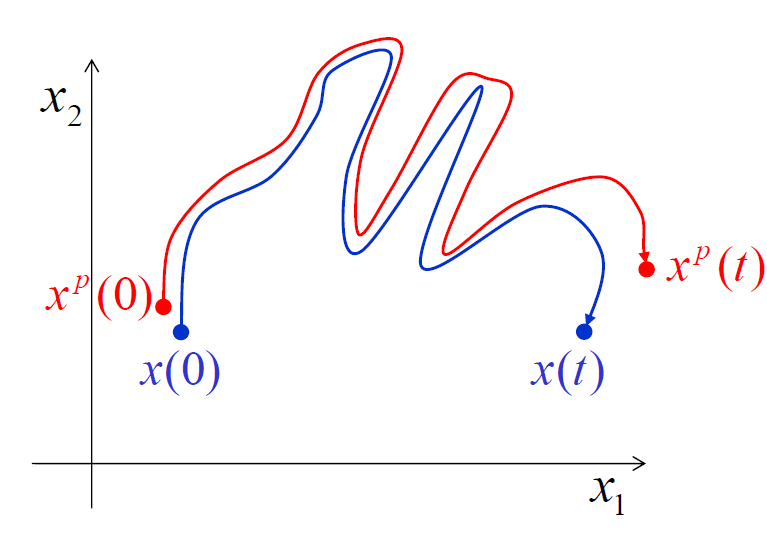
\includegraphics[scale=0.6]{NonLinearControl/images/NominalPerturbed.png}
    \caption{{\color{blue}Nominal solution} and {\color{red}Perturbed solution}} 
    \label{fig:enter-label}
\end{figure*}

\vspace{1cm}
\subsection{Marginal Stability}
\noindent
\textbf{Definition} \textit{(Marginal Stability)} The solution $x(t)$ is \textbf{marginally} (or simply) \textbf{stable} if 
\begin{equation*}
    \forall \epsilon>0, \exists \delta>0 : \\
    \forall x^p(0): \lVert x^p(0)-x(0) \rVert < \delta \Longrightarrow   \lVert x^p(t)-x(t) \rVert < \epsilon, \quad \forall t \ge 0
\end{equation*}
\noindent
{
    \color{blue}
    [Roughly speaking we say that the perturbed solution is always near the nominal solution and so, using other words,  for any choice of $\epsilon$, I am able to find a $\delta$ such that if I choose a perturbed state within the ball of radius $\delta$ for each time $t$, the perturbed solution "fall" within the ball of radius $epsilon$.]
}
\begin{figure}[h]
    \centering
    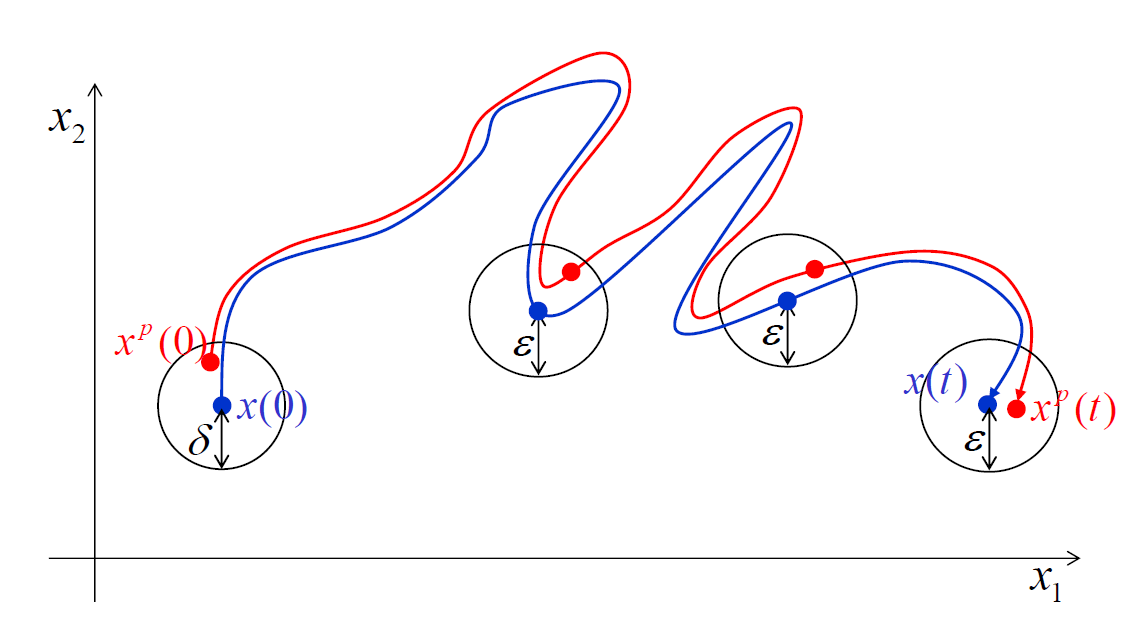
\includegraphics[scale=0.6]{NonLinearControl/images/Stable.png}
    \caption{Marginal stability}
    \label{fig:enter-label}
\end{figure}

\subsection{Asimptotical Stability}
\noindent
\textbf{Definition} \textit{(Asimptotical stability)} The solution $x(t)$ is \textbf{asimptotically stable} if is stable and 
$\lim_{t\to\infty} \lVert x^p(t)-x(t) \rVert=0$. Moreover if the convergence is \textbf{exponential}, the solution is \textbf{exponentially stable}. (This concept is also linked to \textit{modal analysis}.)

\begin{figure}[h]
    \centering
    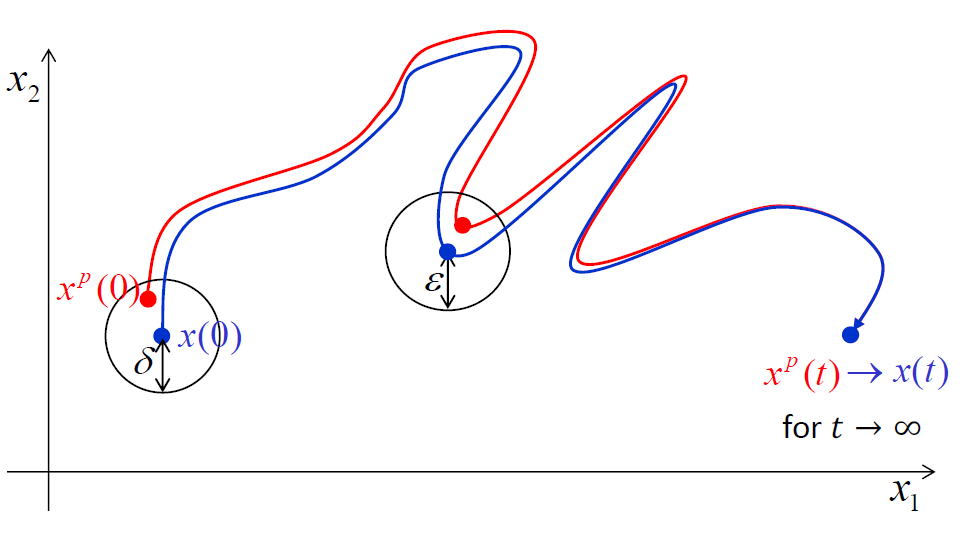
\includegraphics[scale=0.6]{NonLinearControl/images/AsStable.png}
    \caption{Asimptotical stability of a trajectory}
    \label{fig:enter-label}
\end{figure}

\subsection{Unstability}
\noindent
\textbf{Definition} \textit{(Unstability)} A solution of a system is \textbf{unstable} if it is not stable. (Despite I  choose a perturbed initial condition which could be even very close to $x(0)$, the perturbed solution $x^p(t)$ \textbf{go far away} from $x(t)$.

\begin{figure}[h]
    \centering
    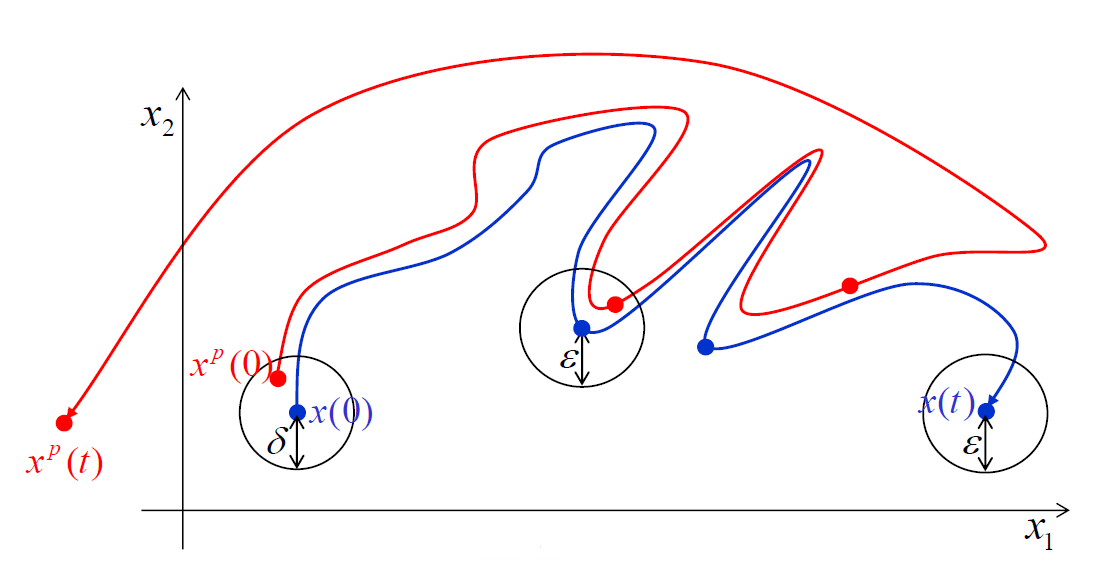
\includegraphics[scale=0.6]{NonLinearControl/images/Unstable.png}
    \caption{Unstable solution}
    \label{fig:enter-label}
\end{figure}

\section{Equilibrium point of a system}

\subsection{Equilibrium point} Given a system with the state equation $\dot{x}=f(\bar{x},\bar{u})$, given a constant input $\bar{u}$, \textbf{$\bar{x}$} is called an \textbf{equilibrium point or state} corresponding to the constant input \textbf{$\bar{u}$}, if it is solution of the equation $$f(\bar{x}, \bar{u})=0$$

\noindent
\textbf{So:} $f(\bar{x}, \bar{u})=0 \Longleftrightarrow \dot{x}=0 \Longleftrightarrow \textrm{null variation over the time} \Longleftrightarrow \textrm{the state remains constant}$

\subsection{Stability of the equilibrium point}

\textbf{Definition} (Stability) The equilibrium point $\bar{x}$ is stable if: 
\begin{equation*}
    \forall \epsilon, \exists \delta: \forall x(0): \lVert x(0)-\bar{x} \rVert \le \delta \Longrightarrow \lVert x(t)-\bar{x} \rVert \le \epsilon, \quad \forall t \ge 0
\end{equation*}
\begin{figure}[h]
    \centering
    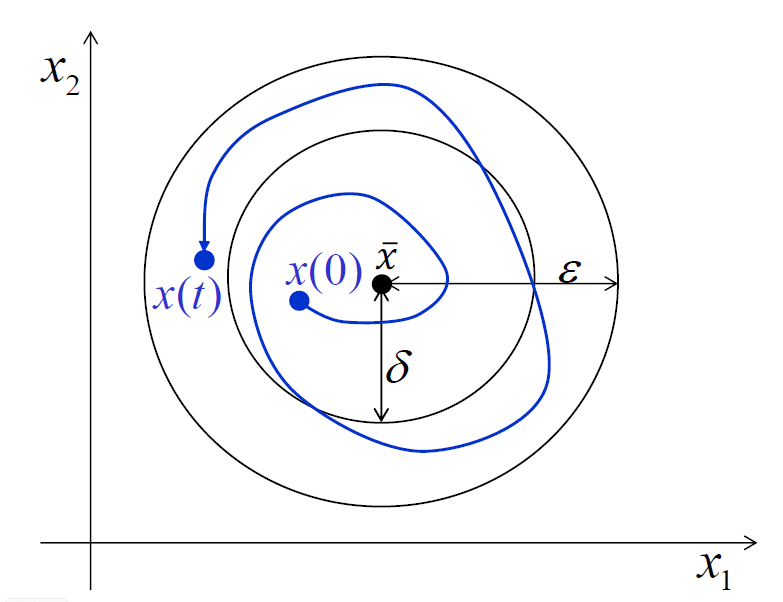
\includegraphics[scale=0.5]{NonLinearControl/images/EqStable.png}
    \caption{Stable equilibrium point}
    \label{fig:enter-label}
\end{figure}

\noindent{
\color{blue}
    A \textbf{simpler explanation} of this concept is that if we move from the equilibrium point choosing a $x(0)$ within a certain ball of radius $\delta$, the equilibrium point itself is stable if the trajectory $x(t)$ remains close to the equilibrium point within another ball of a certain radius $\epsilon$.\\
    
    To find the equilibrium point is sufficient to solve the equation $f(\bar{x}, \bar{u})=0$. Sometimes is quite easy to solve it (e.g. the case of the pendulum), but many times could be not trivial to find an analytical solution.  \\
} 

\noindent
\textbf{Definition} (Asymptotic Stability) The equilibrium state $\bar{x}$ is \textbf{asymptotically stable} if it is stable and it holds that: $$\lim_{t\to \infty} \lVert x(t)-\bar{x} \rVert =0$$

\begin{figure}[h]
    \centering
    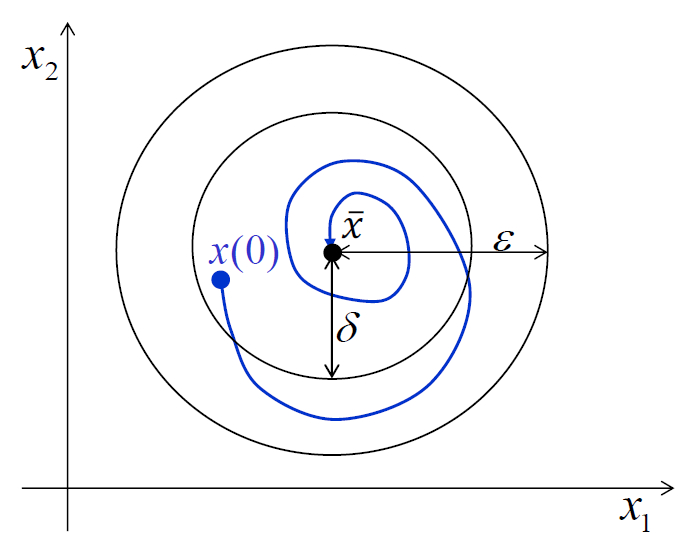
\includegraphics[scale=0.55]{NonLinearControl/images/EqAsStable.png}
    \caption{Asymptotically stable equilibrium point}
    \label{fig:enter-label}
\end{figure}

\noindent
\textbf{Definition} (Instability) The equilibrium state $\bar(x)$ is unstable if it is not stable. That is, Despite we remain close to the equilibrium point the trajectory goes far away the neighbourhood of the point itself.

\begin{figure}[h]
    \centering
    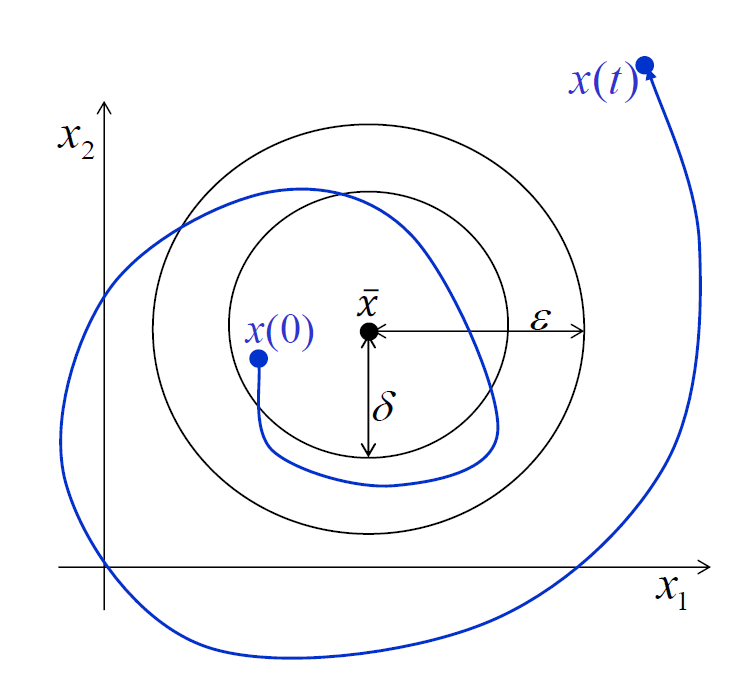
\includegraphics[scale=0.5]{NonLinearControl/images/EqUnstable.png}
    \caption{Unstable equilibrium point}
    \label{fig:enter-label}
\end{figure}

\vspace{1cm}
\noindent
\textbf{Definition} (Domain of attraction) \textbf{A domain of attraction} is a (generic) set of points such that the trajectories initiated at these point converge to the \textit{equilibrium point}. \textbf{The domain of attraction} is the set of \textbf{all points} such that if we start from these point we reach the equilibrium point. If asymptotic stability holds for all initial conditons, then the equilibrium point is \textbf{stable in the large} or \textbf{globally} stable.

\section{Particular case: Stability of LTI systems}
In the case of a Linear Time-Invariant (LTI) system we can write the state solution as $\dot{x}(t)=Ax(t)+Bu(t)$. In this particular case the stability is for the system, not only for a trajectory.\\
For any constant input $\bar{u}$ the equilibrium states can be found \textbf{solving respect to $\bar{x}$} the equation
\begin{equation*}
    \dot{x}=A\bar{x}+B\bar{u}=0 \longleftrightarrow 
    A\bar{x}=-B\bar{u}
\end{equation*}
If $det(A)\ne 0$, then the solution is unique otherwise we can have infinite solutions which generate a subplane (e.g. a line). In the case that $\bar{u}=0$ we obtain a subspace.\\
If $\lambda_1,..., \lambda_i$ are the  \textbf{eigenvalues} of A and $k_1,..., k_i$ are their \textbf{auxiliary geometric multiplicities}, holds that: \\

\noindent
\textbf{Theorem} The LTI system is (internally):
\begin{enumerate}
    \item {\color{red} asymptotically stable} stable if and only if
    $Re(\lambda_i)<0, \forall i$
    \item{\color{red} marginally stable } if and only if $Re(\lambda_i)\le 0, k_i=1 if Re(\lambda_i)=0$
    \item {\color{red} unstable} if and only if
    $\exists i: Re(\lambda_i)>0 \quad \textrm{or} \quad \exists i: Re(\lambda_i)=0, k_i>1$
\end{enumerate}

\noindent
In the case of \textit{non linear systems} the results which has just seen have to be applied to \textbf{each equilibrium point}. It is also of interest to analyze a general property of stability which is the \textbf{BIBO stability} (Bounded Input - Bounded Output), that refers to any type of system of the form 
\begin{align*}
    &\dot{x}=f[x, u, t]\\
    &y=h[x, u, t]
\end{align*}

\noindent
\textbf{Definition} (BIBO stability) A system descripted by the standard state equation  is \textbf{BIBO stable} if \textbf{for any bounded initial condition} and \textbf{for any bounded input} such that $\lVert u(t) \rVert \le M_u < \infty, \forall t \ge 0$ the resulting output is also bounded, that is $\lVert y(t) \rVert \le M_y, \forall t\ge 0$

\noindent
In order to conclude this chapter, we can mention some observation that come from the \textit{modal analysis}: 
\begin{itemize}
    \item asympotic stability $\Longrightarrow$ BIBO stability
    \item BIBO unstability $\Longrightarrow$ instability or marginal stability
\end{itemize}
An example of system that is (simply) stable but NOT BIBO stable is the integrator descripted by the equation
$$\dot{x}(t)=u(t), \quad y(t)=x(t), x,y,u \in \mathbb{R}$$
If we applied a \textbf{constant input} the result \textbf{y(t)} is a ramp. Moreover the BIBO stability is also called \textbf{external stability}.






\chapter{Behaviour of Non Linear systems}

The \textbf{behaviours} of non linear systems can be differ a lot from the linear one. The first difference we observed was that while for an LTI system we can say that \textbf{the system is stable} (stability as a property of the system), for non linear systems we talk about \textbf{the stability of a trajectory (or solution)} (stability as a property of a particular solution $x(t)$ of the system). \\
The phenomena which occurs in the case of non linear system are for example: \begin{itemize}
    \setlength\itemsep {0em}
    \item multiple isolated equilibrium points (see the example)
    \item limit cycles
    \item bifurcations
    \item finite escape time
    \item chaos
    \item ...
\end{itemize}

\section{Phase plane portrait}
We focus in this part on \textbf{Second-Order systems}, that are those for which $n_x=2$. The \textbf{phase plane analysis} is a method for studying the properties of such systems, for higher dimensions we can use a sort of generalization represented by the \textit{Poincare Maps}.\\
The analysis we conduct reguard the \textbf{free evolution} of the system, and it is done in order to understand the most intrinsic properties of the system itself.   \\

\noindent
\textbf{Definition} (Phase Portrait, in Italian "Ritratto di fase") Let us consider an \textit{autonomous system} with state $x=(x_1, x_2)\in\mathbb{R}^2$: $\dot{x}(t)=f(x)$, but we can write it also as: 
\begin{align*}
    &\dot{x_1}=f_1(x_1, x_2)   \\
    &\dot{x_2}=f_2(x_1, x_2)
\end{align*}
For any initial condition $x(0)$ the integration of the equation generates a solution and consequently a trajectory. If we repeat the integration for different $x(0)=x_0$ we obtain a family of trajectories which is called {\color{red} \textbf{phase portrait}}.\\

\noindent
\textbf{Example} (Mass-Spring-Damper)\\
Let us consider a \textbf{mass-spring-damper} system with $F=0, \quad \beta=0,\quad m=1,\quad k=1$. The dynamic equation of the system is $\ddot{p}+p=0$, it has solution: $p(t)=p_0 \cos t$ and $\dot{p}(t)=-p_0 \sin t$. We have in this case $x_1=p(t)$ and $x_2=\dot{p(t)}$. \\
We can determine a well known relation between the two variables that we can plot in the \textit{phase plane} or \textit{state domain}. This equation is: $p^2+\dot{p}^2=p_0^2$ which defines a circle of radius $p_0$ in the phase plane. Varying $p_0$ we obtain the \textbf{phase portrait} representation.

\begin{figure}[h]
    \centering
    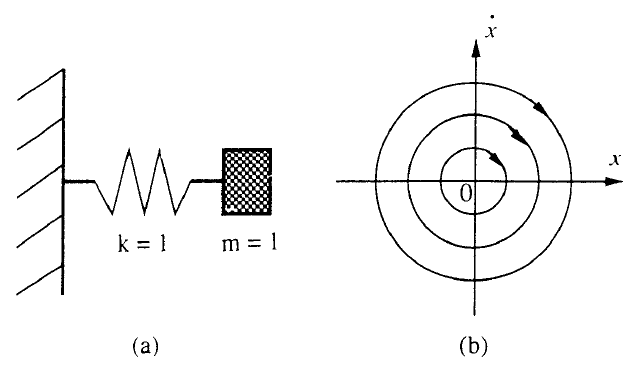
\includegraphics[scale=0.7]{NonLinearControl/images/PhasePort_MSD.png}
    \caption{Mass-Spring-Damper and its \textit{phase portrait}}
    \label{fig:enter-label}
\end{figure}

\subsection{Singular Points} 
Given the system $\dot{x}=f(x)$ with $x \in X \subseteq \mathbb{R}^2$. We define the \textbf{slope} of a trajectory at a point $x=(x_1, x_2)$ as: $$\frac{dx_2}{dx_1}=\frac{f_2(x_1, x_2)}{f_1(x_1, x_2)}$$
At this point we can distinguish \textbf{two cases}: 
\begin{itemize}
    \item $f_2(x_1, x_2)\ne 0, f_1(x_1, x_2)\ne 0$ in this case the slope is \textbf{well defined} and the trajectories won't intersect in the phase plane; 
    \item $f_2(x_1, x_2)=f_1(x_1, x_2)=0$ we can't define the slope that is \textbf{undetermined}, and so some trajectories intersect at point $x=(x_1, x_2)$. We call this point \textbf{singular (or fixed) point}.
\end{itemize}

\noindent
\textbf{Important!} As in the case of the \textit{singular points} we assume that $\dot{x_1}=f_1=0 $ and $\dot{x_2}=f_2=0$ follows that the points for which this happen, are also \textbf{equilibrium points}. They are stable if all trajectory \textbf{converge} to this equilibrium point.

\begin{figure}[h]
    \centering
    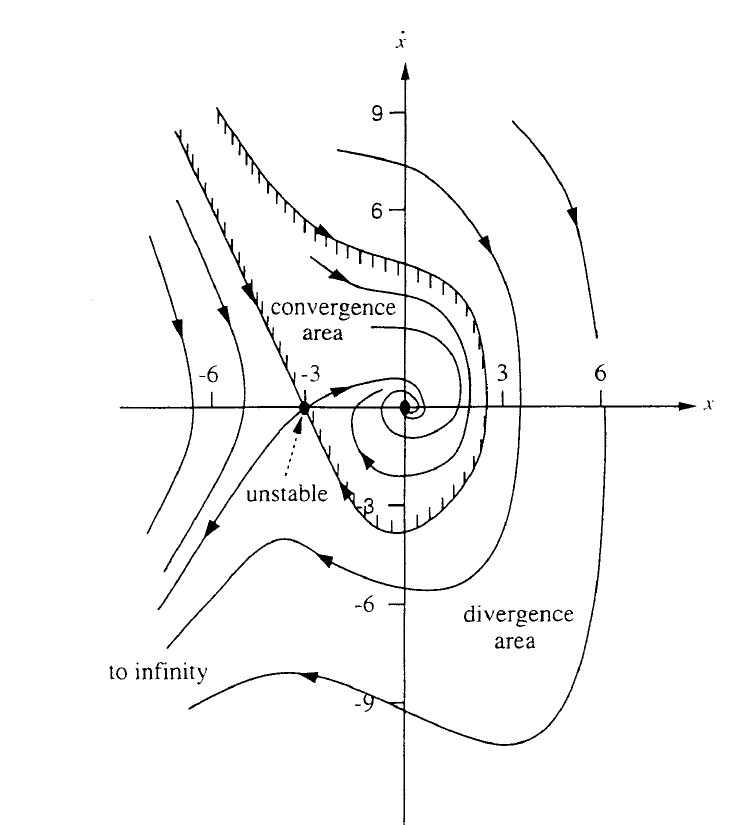
\includegraphics[scale=0.55]{NonLinearControl/images/SingularPoints.png}
    \caption{The phase portrait of a Non Linear System}
    \label{fig:phase}
\end{figure}

\subsubsection{Some considerations}
\begin{itemize}
    \item The Figure \ref{fig:phase} cannot be the phase portrait of an LTI system: in that case we have either one or infinity equilibrium points. This highlight that in the non linear case there can exist few isolated equilibrium points;
    \item In the figure there are two equilibrium point: one is \textit{stable} another is \textit{unstable}.
    \item The figure is the phase portrait linked to the following example:
    \begin{figure}[h]
        \centering
        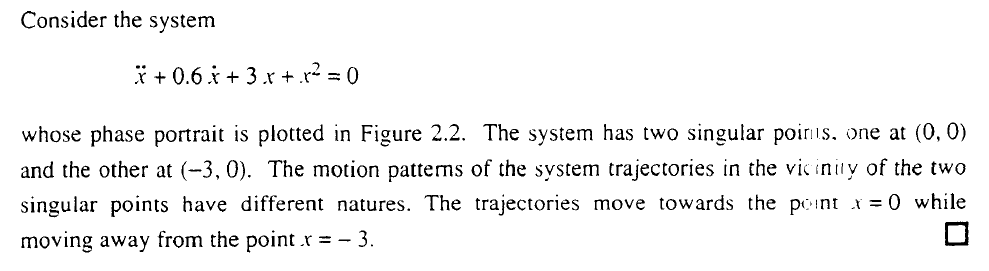
\includegraphics[scale=0.8]{NonLinearControl/images/Slotine1.png}
        \label{fig:enter-label}
    \end{figure}
\end{itemize}

\noindent
It is interesting to note that a phase portrait might by drawn even for a \textbf{first order system}, the difference is that we would have only one trajectory on which we can choose the initial condition. We show here an example (from book "Applied non linear control" - Slotine, 1996): 
\begin{figure}[h]
    \centering
    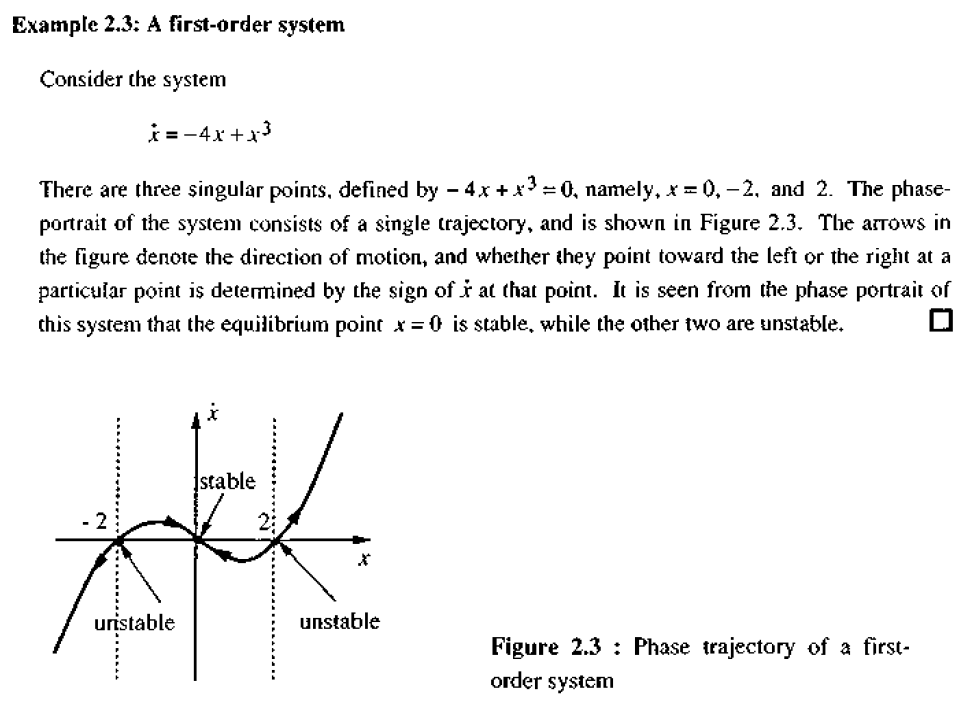
\includegraphics[scale=0.8]{NonLinearControl/images/ExFirstOrder.png}
    \caption{Example of first order phase portrait}
    \label{fig:enter-label}
\end{figure}


\subsection{Methods to draw phase portrait}
There are mainly \textbf{two methods} for constructing the \textit{phase portrait}: 
\begin{enumerate}
    \item \textbf{Analytical/Geometrical methods}: they can be applied only in particular cases; 
    \item By using \textbf{Numerical simulation}: can be applied in any case, moreover they can be generalized to system of order higher than 2.
\end{enumerate}

\section{Behaviour of LTI systems}
Studying the phase portrait of \textbf{LTI systems} is important because: i) we can have an idea of their behaviour, ii) We can use them to study locally the (continuous) non-linearities. We are talking about systems of the form $\dot{x}=Ax$ which have quite simple properties: 
\begin{enumerate}
    \item An LTI system has a \textbf{unique equilibrium point} if the matrix A is non-singular, such point is stable if the eigenvalues of the A matrix have strictly negative real part, \textit{regardless the initial conditions}; 
    \item The solutions can be computed analitically in an easy way; 
    \item In presence of an input $ut(t) \ne 0$ the system becomes of the form $\dot{x(t)}=Ax(t)+Bu(t)$ and we can observe that: 
    \begin{enumerate}
        \item We can apply the \textbf{superposition princple }; 
        \item The asimptotic stability leads to BIBO stability
        \item If $u(t)=A\sin(\omega t + \phi)$, the output is a sinusoidal signal of the same frequency and (Magnitude, Phase) depending on the transfer function of the system itself.
    \end{enumerate}
\end{enumerate}

In order to give consider the case when $A\in \mathbb{R}^{2,2} \quad x \in \mathbb{R}^2$, the system has got \textbf{two eigenvalues} $\lambda_1, \lambda_2$. Actually, we can distinguish the following cases:
\begin{enumerate}
    \item \textbf{$\lambda_{1, 2}$ with the same sign (node)}, if they are both negative, all solution converge otherwise all diverge; 
    \begin{figure}[h]
        \centering
        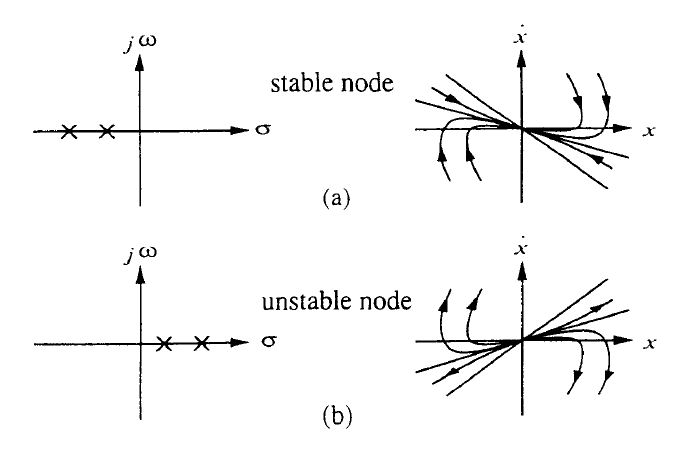
\includegraphics[scale=0.8]{NonLinearControl/images/node.png}
        \caption{Stable/Unstable Node }
        \label{fig:enter-label}
    \end{figure}
    
    %----------------------------------------------
    \item \textbf{$\lambda_{1, 2}$ with opposite signs (saddle)}, in this case as we have some positive, some negative eigenvalue $\Rightarrow$ some solutions converge other diverge; 
    
    \begin{figure}[h]
        \centering
        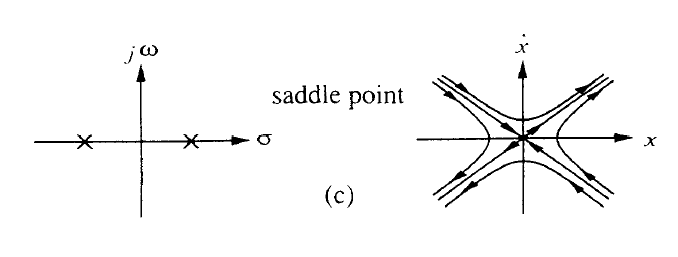
\includegraphics[scale=0.8]{NonLinearControl/images/saddle.png}
        \caption{Saddle point}
        \label{fig:enter-label}
    \end{figure}
     %----------------------------------------------
    \item \textbf{$\lambda_{1, 2}$ complex conjugate with non-zero real part (focus)} in this case if $\textrm{Re}(\lambda_{1,2})<0$ the solutions converge, if $\textrm{Re}(\lambda_{1, 2})>0$, the solutions diverge.
    \begin{figure}[h]
        \centering
        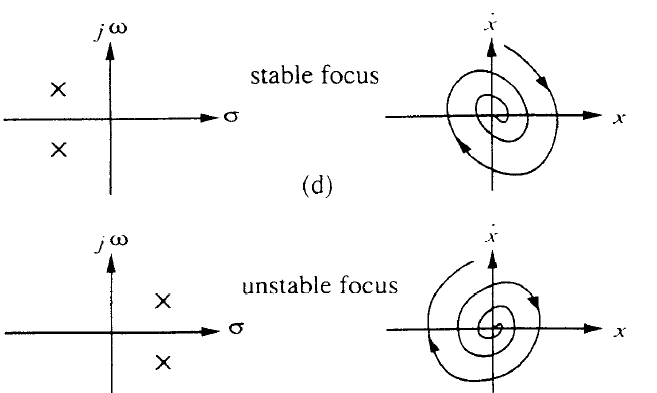
\includegraphics[scale=0.8]{NonLinearControl/images/focus.png}
        \caption{Caption}
        \label{fig:enter-label}
    \end{figure}
    
     %----------------------------------------------
    \item \textbf{$\lambda_{1, 2}$ complex conjugate with zero real part (center)} some  trajectories are \textbf{ellipsis} as they are composition of harmonic signals; 

    \begin{figure}[h]
        \centering
        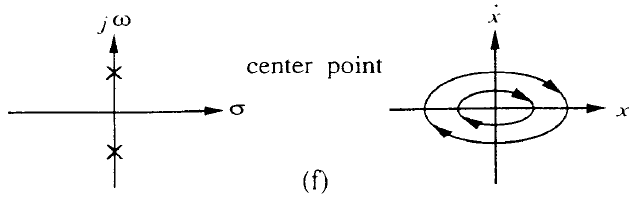
\includegraphics[scale=0.8]{NonLinearControl/images/center.png}
        \caption{Caption}
        \label{fig:enter-label}
    \end{figure}
\end{enumerate}


\section{Non linear case}
The \textbf{behaviour of non linear systems} is much more complex, due to the lack of linearity and superposition principle, they respond to external inputs in a different way. Next we enumerate the most common behaviours: multiple equilibrium points, limit cycles, bifurcations, finite escape time, chaos...

\subsection{Multiple isolated equilibrium points}
Some non linear systems (e.g. the pendulum) have multiple equilibrium points which are isolated, that is in the vicinity there no other equilibrium points. As we said before in the case of LTI systems there only two possibilities: (1) \textbf{a single equilibrium point}, (2) infinitely many equilibrium points in the case that $\textrm{det}(A)=0$.

\subsection{Limit cycles}
A \textbf{limit cycle} is an \textbf{isolated closed curve} on which the motion is \textit{periodic}. A famous example is the \textbf{Van Der Pol oscillator} which is substantially a mass-spring-damper system with a non linear damper.\\
\textit{Limit  cycles} are unique properties of non linear systems, the limit cycle has to be both:
\begin{enumerate}
    \item \textbf{closed}, this feature indicate the periodic motion
    \item \textbf{isolated}, with nearby trajectories that converge or diverge from it.
\end{enumerate}
Depending on the motion of the trajectories in the vicinity of the limit cycle, it can be called:
\begin{itemize}
    \item \textbf{Stable limit cycle}: all trajectories in the "neighbourhood" converge to it $\rightarrow$ we have an \textbf{ATTRACTOR}; 
    \item \textbf{Unstable limit cycle}: all trajectories diverge from the limit cycle $\rightarrow$ we have a \textbf{REPELLOR}; 
    \item \textbf{Semi-Stable limit cycle}: some trajectories converge to it, other diverge $\rightarrow$ we have a \textbf{SADDLE}; 
\end{itemize}

\begin{figure}[h]
    \centering
    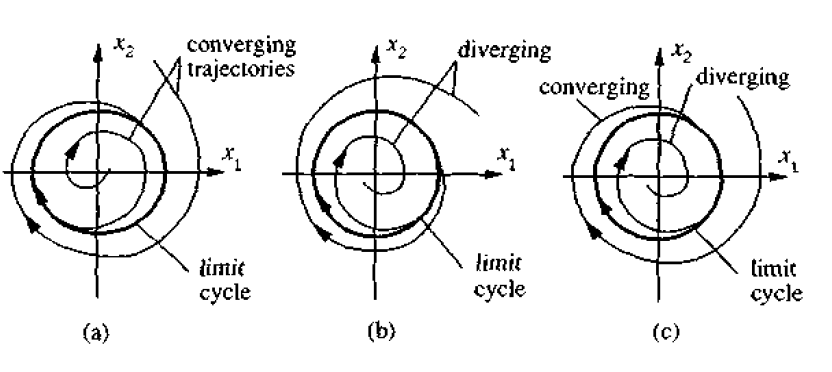
\includegraphics[scale=0.7]{NonLinearControl/images/limitcycles.png}
    \caption{Types of \textbf{limit cycles}}
    \label{fig:enter-label}
\end{figure}
The limit cycle of a \textit{Van Der Pol} oscillator is a stable one.\\
Limit cycles represent an important phenomenon in non linear systems as they can be encountered in many engineering applications and in nature. To give an example in the Aerospace field a limit cycle caused by the interaction between \textit{aerodynamic forces} and \textit{structural vibrations} can be very dangerous. Other times a limit cycle could be desirable! An engineer has to know \textbf{how to eliminate them} when undesirable, how to \textbf{create/amplify} them when they give some advantages. There are some \textbf{simple theorems} that provide a method to individuate them by analyzing some mathematical properties of the system.

\subsubsection{Tori}
When the order of the system is that $n_x>3$, than the motion in the state space can occur on a Torus which constitute a generalization of non-isolated cycle (pendulum) or limit  cycles in \textit{higher dimension}, for this reason, it can be an attractor, repellor or saddle.

\subsection{Bifurcations}
When the \textbf{physical parameters} of a system change, can change also the equilibrium points combined with their stability properties. The values of the parameters ($\alpha$) in general for which this variations occurs are called \textbf{critical} or \textbf{bifurcation values}.\\
The \textbf{bifurcation}, i.e. the \textbf{quantitative change of the parameters} resulting in a \textbf{qualitative change of the system} is another property which characterize non linear systems.\\
Common examples are \textbf{pitchfork} and \textbf{Hopf} bifurcations.

\subsection{Finite escape time}
Is a phenomenon by which some states diverge in a finite time we call $t_esc$, that is equivalent to state that $\lim_{t\to\infty}x(t)=\infty$.

\section {Chaotic systems}
For LTI systems, small differences in initial conditions can cause small differences in the output. For non linear systems is different: there are many cases in which a \textbf{small difference in the initial conditions} is able to lead to \textbf{unpredictable behaviours}, this phenomenon is called \textbf{chaos}. It is useful to distinguish chaos from random motion, in the case of \textit{chaos} the problem is deterministic and there is a small uncertainty in the initial conditions.\\
Chaotic behaviours can be observed in many physical systems (e.g. the \textbf{atmosphere model} can be described like this), the most common is the \textbf{turbulence} in fluid mechanics.\\
In the context of \textbf{feedback control} it  is important to recognize when a system can enter in a chaotic behaviour, and techniques to recover the system itself from it are required.
The motion on these systems can occur over geometric entities with \textbf{fractal structures} called \textbf{strange attractors}, besides you can have \textbf{strange repellors} and \textbf{strange saddles}. Their dimensions are measured by using the \textbf{Housdorff dimensions}. \\

One of the classical \textbf{academic examples} is the \textit{Chua circuit}, which is a quite simple electrical circuit with a non linear resistor whose trajectories are strange attractors. The figure shows two different solutions with different initial conditions.

\begin{figure}[h]
    \centering
    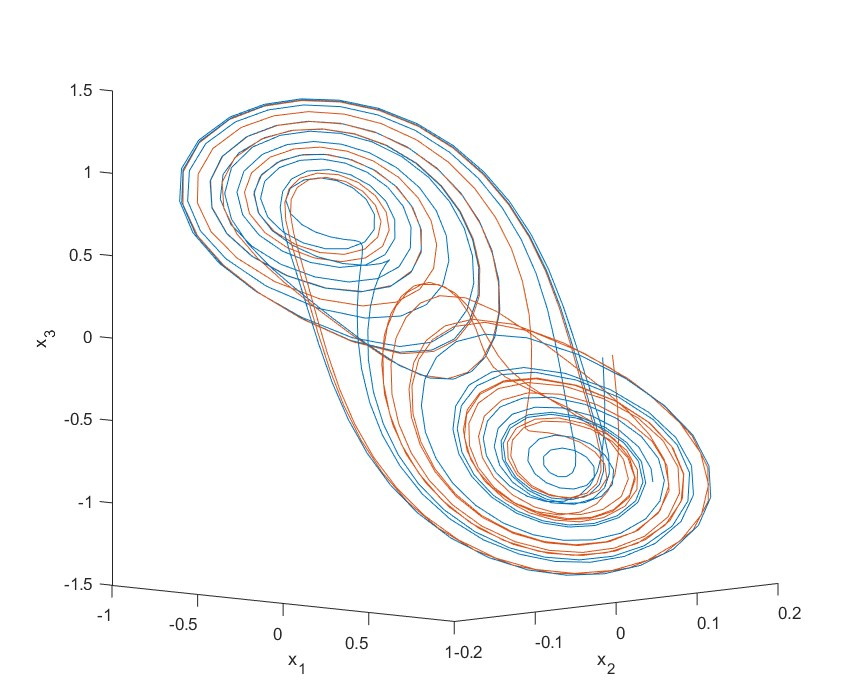
\includegraphics[scale=0.36]{NonLinearControl/images/chuaAttr.jpg}
    \caption{Strange attractor for the \textit{Chua Circuit }}
    \label{fig:enter-label}
\end{figure}

\begin{figure}[h]
    \centering
    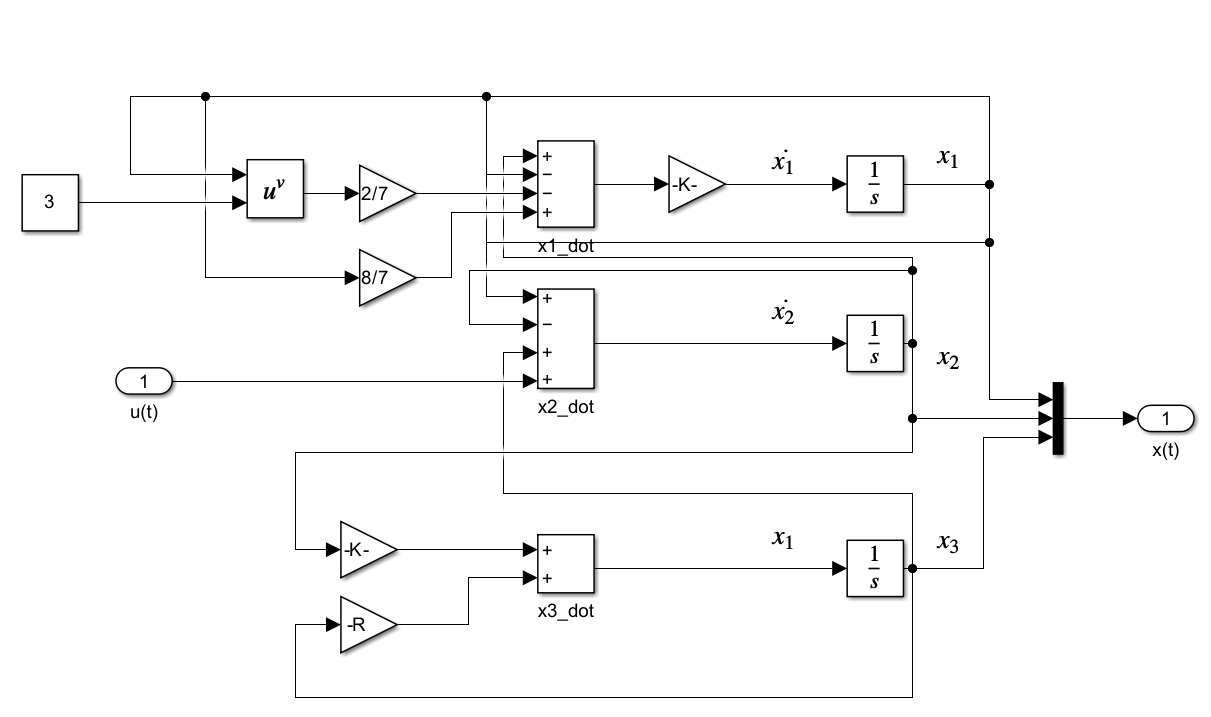
\includegraphics[scale=0.5]{NonLinearControl/images/slk_model.png}
    \caption{Simulink model for the Chua Circuit}
    \label{fig:enter-label}
\end{figure}



\chapter{Lyapunov methods for non linear systems}  
\textit{Aleksandr Michajlovic Lyapunov} (1857-1918) proposed two methods to study the stability of a \textbf{non linear system}. The first is based on observations done on a \textbf{linearized system}, the second is based on seeking a particular function that could satisfy some properties.

\section{Linearization method (LM)}
It is often of interest to linearize a system either around an \textbf{equilibrium point} or a \textbf{trajectory}. Usually it is useful to analyze the system and control it in a proper way.\\
A non linear system has the form 
\begin{align*}
    &\dot{x(t)}=f[x(t), u(t)]\\
    &y(t)=h[x(t), u(t)]
\end{align*}
In this scenario we define the following quantities:
\begin{align*}
    &\delta x(t) = x(t)-\bar{x}\\
    &\delta u(t) = u(t)-\bar{u}\\
    &\delta y(t)=y(t)-h(\bar{x}, \bar{u})
\end{align*}

The \textbf{linearization step} is based on the \textbf{Taylor expansion} which states that \textbf{in the neighbourhood of an equilibrium point $x_0 $}, $$ f(x) = f(x_0)+\frac{\partial f}{\partial x} (x-x_0)$$
If we apply this result to the non linear system for both functions $f$ and $g$ we obtain: 
\begin{align*}
    \dot{x}= f(x,u) =\delta \dot{x}(t) &= 
        \frac{\partial f}{\partial x} \Bigg|_{(\bar{x}, \bar{u})} \delta x +
        \frac{\partial f}{\partial u} \Bigg|_{(\bar{x}, \bar{u})} \delta u\\
    \delta y(t) &= \frac{\partial h}{\partial x} \Bigg|_{(\bar{x}, \bar{u})} \delta x +
    \frac{\partial h}{\partial u} \Bigg|_{(\bar{x}, \bar{u})} \delta u
\end{align*}
Due to the fact that $f(x,u)$, $h(x,u)$ are \textbf{vector fields} the derivatives are \textbf{Jacobian matrices} which corrensponds to matrices $A, B, C, D$ of a linearized system
\begin{align*}
    &\delta \dot{x}(t)=A\delta x(t) + B \delta u(t)\\
    &\delta y(t) = C \delta x(t) + D \delta u(t)
\end{align*}
Where the matrices $A, B, C, D$ are defined as follows:
{
    \large{
        \begin{align*}
            &A = \begin{bmatrix}
                \frac{\partial f_1}{\partial x_1} & \ldots & \frac{\partial f_1}{\partial x_{n_x}} \\
                \vdots                            & \ddots &  \vdots \\
                \frac{\partial f_{x_n}}{\partial x_1} & \ldots & \frac{\partial f_{x_n}}{\partial x_{n_x}}
            \end{bmatrix}_{(\bar{x}, \bar{u})} \quad
            B = \begin{bmatrix}
                \frac{\partial f_1}{\partial u_1} & \ldots & \frac{\partial f_1}{\partial x_{n_u}} \\
                \vdots                            & \ddots &  \vdots \\
                \frac{\partial f_{x_n}}{\partial u_1} & \ldots & \frac{\partial f_{n_u}}{\partial x_{n_x}}
            \end{bmatrix}_{(\bar{x}, \bar{u})}\\
            &C = \begin{bmatrix}
                \frac{\partial f_1}{\partial x_1} & \ldots & \frac{\partial f_1}{\partial x_{n_x}} \\
                \vdots                            & \ddots &  \vdots \\
                \frac{\partial f_{x_n}}{\partial x_1} & \ldots & \frac{\partial f_{x_n}}{\partial x_{n_x}}
            \end{bmatrix}_{(\bar{x}, \bar{u})}  \quad
            D = \begin{bmatrix}
                \frac{\partial f_1}{\partial x_1} & \ldots & \frac{\partial f_1}{\partial x_{n_x}} \\
                \vdots                            & \ddots &  \vdots \\
                \frac{\partial f_{x_n}}{\partial x_1} & \ldots & \frac{\partial f_{x_n}}{\partial x_{n_x}}
            \end{bmatrix}_{(\bar{x}, \bar{u})}
        \end{align*}
    }
}
The \textbf{linearized system} represents an approximation of the non linear system in the neighbourhood of the equilibrium point $(\bar{x}, \bar{u})$
\subsection{Stability of an equilibrium point}
Let $\lambda_1, ..., \lambda_{n}$ be the eigenvalues of the $A$ matrix  previously defined. The \textbf{equilibrium point} $(\bar{x}, \bar{u})$ of the system is:
\begin{itemize}
    \item \textbf{Asimptotically stable} if and only if $\textrm{Re}(\lambda_i)<0 \quad \forall i$
    \item \textbf{Unstable} if exists an $i$ such that $\textrm{Re}(\lambda_i)>0$
    \item Nothing can be said in case of marginal stability of the linearized system. 
\end{itemize}

This method is very simple, but provide us a way to study only the \textbf{local stability}, moreover it does not give any information on stability when the linearized system is only \textbf{marginally stable}.

\section{Lyapunov Direct Method (DM)}
The \textbf{Direct Method (DM)} is not restricted to local motion. It gives a way to determine the stability properties by constructing an \textbf{energy-like function} called the \textbf{Lypunov Function}. The method is based on a \textit{physical observation}: \\

{
\Large{
\centering 
    If the \textbf{total energy} of a system is dissipated, then the  system must settle down to an \textbf{equilibrium point}. 
 }
}\\

For example if we analyze the \textbf{mass-spring-damper} system, we note that is impossible to find an analytical solution, moreover the \textbf{Linearization Method} does not give any useful information if the motion starts outside the linear range. Using instead the expression of \textbf{mechanical energy} we can find more useful information.\\
The \textbf{Lyapunov's Direct Method} is based on a generalization of this idea to more complex systems. Now it is the moment to formalize this concepts and give some useful definitions. \\

 %Per disegnare il box
\hspace*{-5mm}
\begin{tikzpicture}
\node [mybox] (box){%
    \begin{minipage}{.96\textwidth}     %Larghezza del box
            \noindent
\textbf{Definition (Positive definite functions)} A function $V: \mathbb{R}^n  \rightarrow \mathbb{R}$ is \textit{locally positive definite}, if for some ball $B_R=\{x: \lVert x \rVert \le R\}$, 
\begin{align*}
    &V(x)=0, \quad x=0\\
    &V(x)>0, \quad x\ne 0, x \in B_R
\end{align*}
If $B_R=\mathbb{R}^n$ then the function $V(x)$ is said to be \textbf{globally definite positive}.\\
    \end{minipage}
};
\end{tikzpicture}%



\begin{figure}[h]
    \centering
    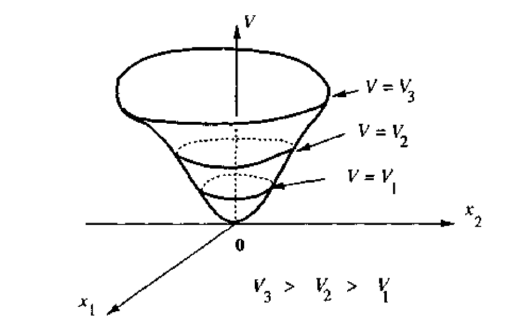
\includegraphics[scale=0.8]{NonLinearControl/images/PD_Fun.png}
    \caption{Example of a \textbf{Positive Definite Function}}
    \label{fig:enter-label}
\end{figure}

    %Per disegnare il box
\hspace*{-5mm}
\begin{tikzpicture}
\node [mybox] (box){%
    \begin{minipage}{.96\textwidth}     %Larghezza del box
            \noindent
\textbf{Definition (Positive semi-definite functions)} A function $V: \mathbb{R}^n  \rightarrow \mathbb{R}$ is \textit{positive semi-definite}, if for some ball $B_R=\{x: \lVert x \rVert \le R\}$, 
\begin{align*}
    &V(x)=0, \quad x=0\\
    &V(x)\ge0, \quad x\ne 0, x \in B_R
\end{align*}
    \end{minipage}
};
\end{tikzpicture}%

\vspace{0.5cm}

    %Per disegnare il box
\hspace*{-5mm}
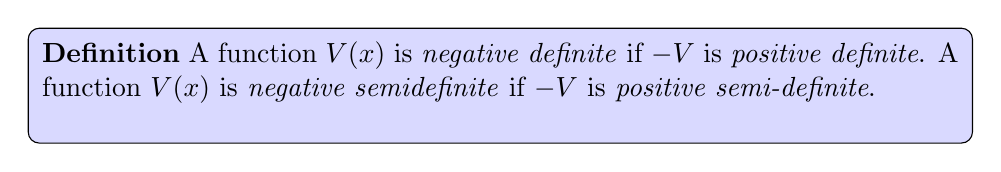
\begin{tikzpicture}
\node [mybox] (box){%
    \begin{minipage}{.96\textwidth}     %Larghezza del box
            \noindent
\textbf{Definition} A function $V(x)$ is \textit{negative definite} if $-V$ is \textit{positive definite}. A function $V(x)$ is \textit{negative semidefinite} if $-V$ is \textit{positive semi-definite}. \\
    \end{minipage}
};
\end{tikzpicture}%



We are ready to give the definition of what is a \textbf{Lyapunov function}, two theorems based on the existence of such function can be used to recover the \textbf{stability properties} of a non linear system.\\

%Per disegnare il box
\hspace*{-5mm}
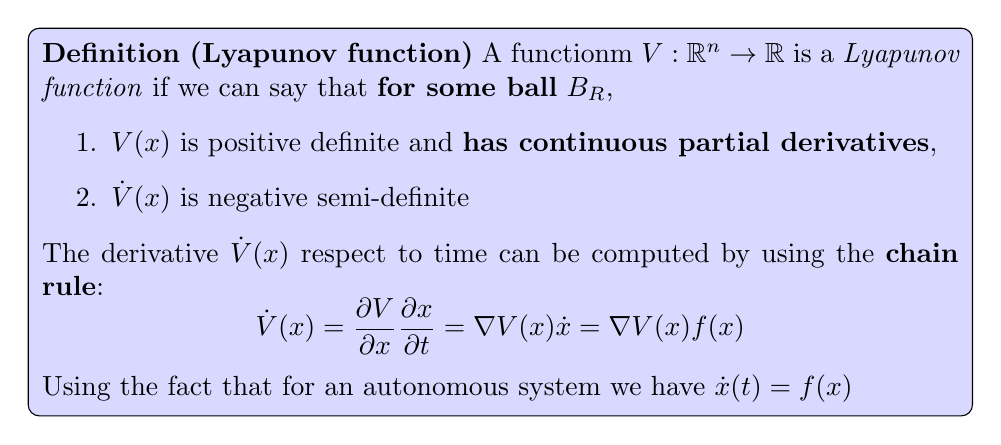
\begin{tikzpicture}
\node [mybox] (box){%
    \begin{minipage}{.96\textwidth}     %Larghezza del box
           \noindent
\textbf{Definition (Lyapunov function)} A functionm 
$V: \mathbb{R}^n \rightarrow \mathbb{R}$ is a \textit{Lyapunov function} if we can say that \textbf{for some ball} $B_R$, 
\begin{enumerate}
    \item $V(x)$ is positive definite and \textbf{has continuous partial derivatives},
    \item $\dot{V}(x)$ is negative semi-definite
\end{enumerate}

The derivative $\dot{V}(x)$ respect to time can be computed by using the \textbf{chain rule}: 
$$
    \dot{V}(x)= \frac{\partial V}{\partial x} \frac{\partial x}{\partial t} = 
    \nabla V(x) \dot{x} = \nabla V(x) f(x) 
$$
Using the fact that for an autonomous system we have $\dot{x}(t)=f(x)$
    \end{minipage}
};
\end{tikzpicture}%

\begin{figure}[h]
    \centering
    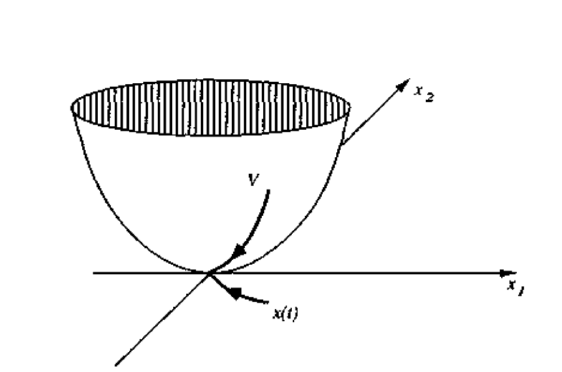
\includegraphics[scale=0.6]{NonLinearControl/images/LyapunovFunction.png}
    \caption{Example of a \textbf{Lyapunov Function}}
    \label{fig:enter-label}
\end{figure}

Without loss of generality we can assume that $\bar{x}=0$ is an equilibrium point, about the stability we have these theorems: \\


%Per disegnare il box
\hspace*{-5mm}
\begin{tikzpicture}
\node [mybox] (box){%
    \begin{minipage}{.96\textwidth}     %Larghezza del box
         \noindent
\textbf{Theorem (local stability)} If the system 
\begin{align*}
    &\dot{x}(t)=f[x(t), u(t)]\\
    &y(t)=h[x(t), u(t)]
\end{align*}
-admits a \textbf{Lyapunov Function} for some ball $B_R$, then the equilibrium point $\bar{x}=0$ is (marginally) stable). \\
-If moreover the function $\dot{V}(x)$ is \textbf{negative definite} in $B_R$ then the stability is  \textbf{asymptotic}.\\
    \end{minipage}
};
\end{tikzpicture}%\\
\vspace{0.5cm}

%Per disegnare il box
\hspace*{-5mm}
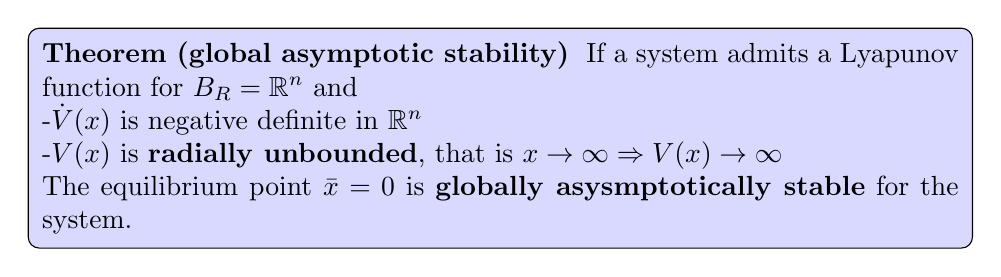
\begin{tikzpicture}
\node [mybox] (box){%
    \begin{minipage}{.96\textwidth}     %Larghezza del box
            \noindent
{\textbf{Theorem (global asymptotic stability)} }
If a system admits a Lyapunov function for $B_R=\mathbb{R}^n$ and \\
-$\dot{V}(x)$ is negative definite in $\mathbb{R}^n$\\
-$V(x)$ is \textbf{radially unbounded}, that is $\lVert x \rVert \rightarrow \infty 
\Rightarrow V(x) \rightarrow \infty
$\\
The equilibrium point $\bar{x}=0$ is \textbf{globally asysmptotically stable} for the system. 
    \end{minipage}
};
\end{tikzpicture}%


\noindent
Such theorems are not constructive,  in the sense that they do not tell us how to build a \textbf{Lyapunov function}, there are some methods that do not allow us to find in general the functions, but only in some cases. Some common methods are:
\begin{itemize}
    \item \textbf{Physical insight approach}, when it is possible to use physical observations a very powerful analysis can be conducted for these systems; 
    \item \textbf{Krasovskii's Method}, it gives \textbf{sufficient conditions} based on the Jacobian of the matrix $A$ of the linearized system. 
    \item \textbf{Variable Gradient Method} where a particular form for the gradient of the function $V(x)$ is assumed, then we compute the $V(x)$ by integrating such gradient.
\end{itemize}

\section {An Example: The pendulum}
In this section are shown an example of \textit{Lyapunov function} for the pendulum case, such function satisfies the properties in the theorem above mentioned. It is: 
\begin{equation*}
    V(x)=2(1-\cos(x_1))+\frac{x_2^2}{2}+\frac{(x_1+x_2)^2}{2}
\end{equation*}
In particular we observe that: 
\begin{enumerate}
    \item $V(x)$ is a Lyapunov Function in a certain ball $B_R$
    \begin{figure}[h]
    \centering
    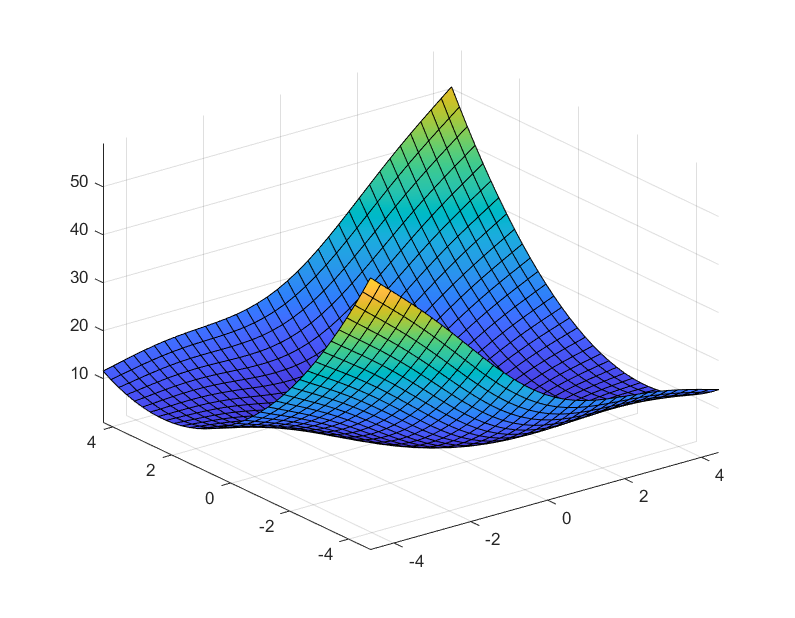
\includegraphics[scale=0.6]{NonLinearControl/images/Lyapunov.png}
    \caption{$2(1-\cos(x_1))+\frac{x_2^2}{2}+\frac{(x_1+x_2)^2}{2}$}
    \label{fig:enter-label}
    \end{figure}
    \item $\dot{V}(x)$ is \textbf{negative definite} in a certain ball $B_R$ centered in $\bar{x}=0$.  
\end{enumerate}

\begin{figure}[h]
    \centering
    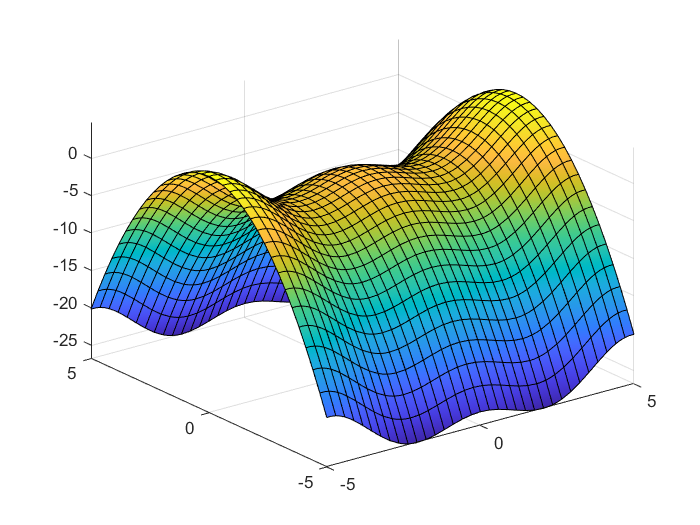
\includegraphics[scale=0.7]{NonLinearControl/images/Lyap_Der.png}
    \caption{$\dot{V}(x)$}
    \label{fig:enter-label}
\end{figure}


\chapter{Introduction to Non Linear Control}
In general the \textbf{control theory} deals with the formulation of a \textbf{control law} $u(t)$ above a given physical system with a given dynamics. The system $C$, the so called \textbf{Controller}, should be applied on the real plant such that $y = r$ for a set of signals of interest. The command $u(t)$ is defined into the system $C$ in a proper way.\\

\begin{figure}[h]
    \centering
    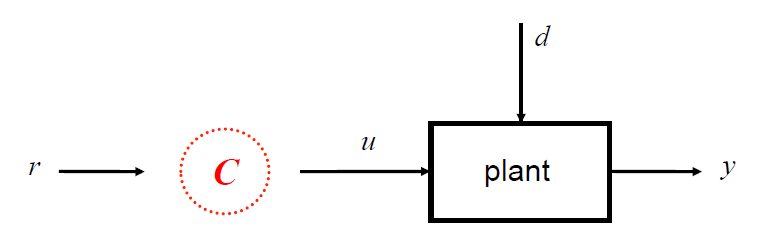
\includegraphics[scale=0.8]{NonLinearControl/images/ControlScheme.png}
    \caption{Classical structure of a controlled plant}
    \label{fig:enter-label}
\end{figure}

\noindent
In this field topics of interest are: (a) The nonlinear stabilization of the real  plant, (b) the nonlinear Tracking, (c) The specification of Desired Behaviour of the System. 

\section{Non linear Stabilization and Tracking}
In the case that the \textbf{tasks of a Control System} involve large range or high speed motions, non linear behaviours and effects can be a problem, for this reason \textbf{non linear control} is necessary to achieve some objectives. \\
Generally speaking, the tasks of a control system can be divided into two categories: 
\begin{itemize}
    \item \textbf{Stabilization} (or Regulation), here a control system called a \textit{stabilizer} (or regulator), is designed so that the \textbf{closed-loop} system is stable around an equilibrium point (examples: temperature regulation, altitude control...);
    \item \textbf{Tracking} (or Servo), here the design objective is to build a controller, called the \textit{tracker}, which has the task to ensure that the system could track a desired \textbf{time-varying trajectory} (examples: making a robot hand draw straight lines or circles, making an aircraft fly along a specified path...)
\end{itemize}

\section{Specifying the desired behaviour}
In linear control, the desired behaviour of a control system can be specified either in the time-domain by providing specifications like rise time, overshoot and settling time) or  in the frequency domain in terms of regions in which the \textit{loop transfer function} (usually indicated with $L(s)$) should lie at high and low frequencies.\\
However, \textbf{systematic specifications} for nonlinear systems (except those equivalent to linear system) are not obvious: at first a frequency-domain specification is not available, the response of the system to one command does not reflect its response to another command. As a result, for nonlinear system, one often try to find some \textbf{qualitative} specifications in the operating region of interest. Some common characteristics are: Stability (guaranteed for the nominal model), Robustness, Cost, Accuracy and speed of response.

\section{A general procedure for Control Design}
Given a physical system to be controlled, one typically goes through the following standard procedure:
\begin{enumerate}
    \item specify the desired behaviour, and select the actuators and sensors; 
    \item model the physical plant by a set of differential equations; 
    \item design a control law for the system;
    \item analyze and simulate the resulting control system;
    \item implement the control system in hardware;
\end{enumerate}

\section{Available methods for nonlinear controllers}
As in the analysis, we have not a general method to \textbf{design a nonlinear controller}, even in this case we have a collection of techniques which are either alternative or complementary and each applicable to a class of nonlinear control problems.\\
\subsection{Trial and error}
It is based on the analysis method provided before, like the \textit{phase plane method} and the \textit{Lyapunov analysis}. The design strategy deploys this technique in a way similar to the loop-shaping. This technique may work sometimes but in complicated situation it fails.

\subsection{Feedback linearization}
As discussed in the previous paragraphs, one of the main steps for design a controller (the first in particular) is to derive a meaningful model for the plant. \textbf{Feedback linearization} deals with techniques for \textit{transforming the original system models into equivalent models of a different simpler form}. Can be used in a proper way as a strategy for design nonlinear controller. The \textbf{basic idea} is to linearize (fully or in part) the nonlinear plant and  then apply the well-known techinques to complete the control design.\\
It is  appliable to a number of practical cases. As a \textit{drawback} it does not guarantee robustness against \textbf{disturbances} and \textbf{parameters uncertainty}.
\subsection{Robust control}
In the great majority of the control techniques the controller is designed according to the \textbf{nominal model of the plant/physical system}. In pure \textbf{model-based} design strategies uncertainties are neglected. In \textbf{robust nonlinear control} (eg. \textit{Sliding Mode Control}), on the other hand, the controller is designed by exploiting both nominal plant and some characterization of the model uncertainties.\\


\subsection{Adaptive control}
\textbf{Adaptive control} is a technique to deal with \textbf{uncertain or time-varying systems}. Despite these alternatives, nowadays, adaptive control techinques are used when one have to face with system with \textit{known dynamic structure} but \textbf{unknown constant or time-varying parameters}. \\
There are quite strong results for linear systems concerning this strategy, but  also for nonlinear systems with \textbf{measurable state} and \textbf{linearly parametrizable dynamics} have been deployed some methods. When it is possible to design such type of controller it represents an alternative or a complementary part for the robust control design. 

\subsection{Gain scheduling}
\textbf{Gain scheduling} is a method which make a try to apply well-known linear techniques to control nonlinear systems. It was developed for the trajectory control of aircraft. \\
The \textbf{idea behind} this technique is to collect a \textbf{set of operating points} which may cover the range of the system operation. Then, at \textbf{each of these points}, the designer makes a linear time variant approximation to the plant dynamics and build a \textbf{linear controller} for each linearized plant. What happen between two operating points? The parameters are interpolated, or \textbf{scheduled}, providing a global compensator. Maybe Gain Scheduling is the simplest method for designing nonlinear controllers, but the main problem is that one have only limited guarantees in stability in non linear operations; another drawback is the necessity of computing a cospicuous number of linear controllers.


\chapter{Method(1): Feedback linearization}
\textbf{Feedback linearization} is an appproach to nonlinear control whose \textbf{central idea} is to algebraically transform a nonlinear system dynamics into a linear one, so that the well-known strategies for linear controllers could be applied. This technique differs from \textit{Jacobian linearization}, in the sense that the \textbf{linearization} is achieved by \textbf{exact} state transformation and feedback, instead of \textit{linear approximation} of the dynamics.\\

This idea of simplifying the form of the system's dynamics by choosing a different \textbf{state representation} is not unfamiliar, it is well known that in mechanics the description could vary a lot according to the choice of the \textbf{reference frame} or \textbf{coordinate system}.  \\

In the introductory discussion of feedback linearization, commonly one give the example of designing a control law for controlling the \textbf{fluid entering into a tank}. Given the dynamics, it is  quite simple to show that can be chosen a particularly simple input to delete the non linearities of the plant in a way that the system resulting in a simple \textbf{integrator}.\\
In more complex situations, than the tank system, it is required to have some standard techniques to linearize the system. In this context we can mention:
\begin{enumerate}
    \item \textbf{input-state linearization} where linearization is performed via state feedback; 
    \item \textbf{input-output} linearization, here linearization is achieved by using the feedback of the output.
\end{enumerate}

To this aim it is useful to introduce the concept of \textbf{Lie derivatives} which is an elegant way to express the well-known \textbf{chain rule}. 
\section{Lie derivatives}
This definitions are given in order to use a more compact notation for the following paragraphs. \\

\hspace*{-5mm}
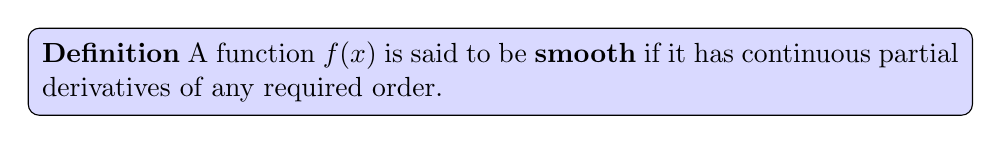
\begin{tikzpicture}
\node [mybox] (box){%
    \begin{minipage}{.96\textwidth}     %Larghezza del box
          \textbf{Definition} A function $f(x)$ is said to be \textbf{smooth} if it has continuous partial derivatives of any required order.
    \end{minipage}
};
\end{tikzpicture}% 

\vspace{0.5cm}
\hspace*{-5mm}
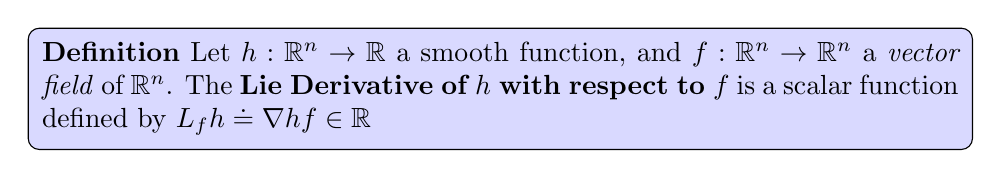
\begin{tikzpicture}
\node [mybox] (box){%
    \begin{minipage}{.96\textwidth}     %Larghezza del box
          \textbf{Definition} Let $h:\mathbb{R}^n\rightarrow \mathbb{R}$ a smooth function, and $f:\mathbb{R}^n\rightarrow\mathbb{R}^n$ a \textit{vector field} of $\mathbb{R}^n$. The \textbf{Lie Derivative of $h$ with respect to $f$} is a scalar function defined by $L_fh\doteq\nabla h f \in \mathbb{R}$
    \end{minipage}
};
\end{tikzpicture}%

\noindent
The meaning of \textbf{Lie derivative} is doing a derivative of $h$ in the direction provided by $f$. The computation of such derivatives can be done in a \textbf{recursive way}, as follows: 
\begin{align*}
    &L_f^0h=h\\
    &L_f^ih=L_f(L_f^{i-1}h)=\nabla(L_f^{i-1}h)f, \quad i=1, 2, ...
\end{align*}

\section{Input-Output linearization}
Now we consider the \textbf{SISO nonlinar system} of the form 
\begin{equation} \label{eq: system_affine}
    \begin{aligned}
        &\dot{x} = f(x)+g(x)u\\
        &y=h(x)
\end{aligned}
\end{equation}

where $x\in\mathbb{R}^{n_x}$ is the state, $u\in\mathbb{R}$ is the command input, $y\in\mathbb{R}$ is the output, and $f$, $g$, $h$ are smooth functions.\\
Such system is said to be \textit{affine in u}. We assume that the state is accessible and so measurable, otherwise an observer has to be employed. \\
\textbf{Input-output linearization} approach consists in differentiate repeatedly, until the input $u$ appears, then design the control law $u(t)$ to cancel the nonlinearity.\\
We can start by taking the output equation $y=h(x)$ and differentiate it: 
\begin{align}
    &\dot{y}=\frac{\partial h}{\partial x}\dot{x}=\nabla h(x)\dot{x}=
    \nabla h(x) (f(x)+g(x)u) = \\
    &\nabla h(x) f(x) + \nabla h(x) g(x) u=
    L_fh+L_gh(x)u
\end{align}
If $L_gh(x) \ne 0$ at some point $x=\bar{x}\in \Omega_x\subseteq\mathbb{R}^n$ then in $\Omega_x$ the control law is: 
\begin{equation}
    u=\frac{1}{L_gh(x)} (-L_fh(x)+v)
\end{equation}
This transforms the output equation in $\dot{y}=v$. Otherwise we differentiate again obtaining: 
\begin{align}
    \ddot{y}=L_f^2h(x)+L_gL_fh(x)u
\end{align}
Until the multiplicative term of $u$ is not null, you have to differentiate again and again obtaining:
\begin{equation}
    y^{(i)}=L_f^{(i)}h(x)+L_gL_f^{(i-1)}h(x)u
\end{equation}
Then, for some $\gamma$ the term $L_gL_f^{\gamma-1}h(x)u \ne 0$ the control law and the resulting system will be respectively\\


\hspace*{-5mm}
\begin{tikzpicture}
\node [mybox] (box){%
    \begin{minipage}{.96\textwidth}     %Larghezza del box
    {
        \large{
         \begin{align}
    &u=\frac{1}{L_gL_f^{\gamma}h(x)}(-L_f^{\gamma-1}+v)\\
    &y^{(\gamma)}=v \label{eq: final_system}
\end{align}}
}
    \end{minipage}
};
\end{tikzpicture}%


The equation (\ref{eq: final_system}) can be written in the state space form, definining the \textbf{state vector}
\begin{equation}
    \mu=(\mu_1,...,\mu_\gamma)\doteq(y, \dot{y},...,y^{(\gamma-1)})
\end{equation}
The resulting state equations are in the so-called \textit{companion form}: \\

\hspace*{-5mm}
\begin{tikzpicture}
\node [mybox] (box){%
    \begin{minipage}{.96\textwidth}     %Larghezza del box
    {
        \large{
         \begin{align*}
    &\dot{\mu}=A\mu+Bv\\
    &y=\mu_1\\
    &A=\begin{bmatrix}
    0&1&0&\dots&0\\
    0&0&1&\ddots&0\\
    \vdots&\vdots&\ddots&\ddots&\vdots\\
    0&0&\dots&0&1\\
    0&0&\dots&0&0
    \end{bmatrix} \quad 
    B=\begin{bmatrix}
        0\\0\\\vdots\\0\\1
    \end{bmatrix}
\end{align*}}
}
    \end{minipage}
};
\end{tikzpicture}%


These equations describe only a part of the system dynamics, called the {\textbf{external dynamics}}, which is the part that one can control. This is linked with another important information of the non linear system that is the \textbf{relative degree}.

\subsection{Relative degree}
Now we give the definition of \textbf{relative degree}:\\

\hspace*{-5mm}
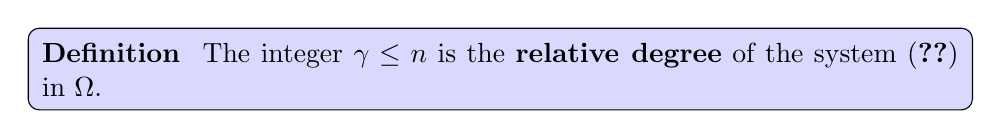
\begin{tikzpicture}
\node [mybox] (box){%
    \begin{minipage}{.96\textwidth}     %Larghezza del box
    \textbf{Definition } The integer $\gamma\le n$ is the \textbf{relative degree} of the system (\ref{eq: system_affine}) in $\Omega$.
    \end{minipage}
};
\end{tikzpicture}% 
\\

 This is a generalization of the concept of relative degree for LTI systems (the difference between the denominator degree and numerator degree of the transfer function $H(s).$
 In the case that $\gamma=n$, input-output linearization corresponds to input-state linearization.\\
 It could happen that the term $L_gL_f^{\gamma-1}h(x)$ is zero at $\bar{x}$ but non zero in the neighbourhood of $\bar{x}$.
 In this case the relative degree is \textit{undefined} in $\bar{x}$.
 
 \subsection{Normal form}
Once we have applied the control law, we can define the \textbf{normal state} $(\mu,\psi)$ in the following way:
\begin{align}
    &\mu=(\mu_1, ..., \mu_\gamma)\doteq (y, \dot{y},..., y^{\gamma-1})\in\mathbb{R}^{\gamma} \quad & \text{external dynamics}\\
    &\psi\in\mathbb{R}^{n-\gamma} & \text{internal dynamics}
\end{align}
The nonlinear system (\ref{eq: system_affine}) can be written in the so called \textit{normal form}:
\begin{equation}
    \begin{aligned}
        &\dot{\mu}=\begin{bmatrix}
            \mu_2\\
            \vdots\\
            \mu_\gamma\\
            a(\mu, \psi)+b(\mu,\psi)u
        \end{bmatrix} \quad \begin{matrix}
            &a(\mu, \psi)\doteq L_f^{\gamma}h(x)\\
            &b(\mu, \psi)\doteq L_gL_f^{\gamma-1}h(x)u
        \end{matrix}\\
        &\dot{\psi}=w(\mu,\psi)\\
        &y=\mu_1
    \end{aligned}
\end{equation}
While the \textbf{external dynamics} is well defined and one can control it, find explicitly the \textbf{internal dynamics} could require to solve Partial Differential Equations (PDE), however in some cases it is possible to study the \textbf{stability of the internal dynamics} theoretically by using the \textit{zero dynamics} otherwise simulations have to be used.
 
\subsection{Zero dynamics}
The internal dynamics of the system (\ref{eq: system_affine}) is not controlled, it can be therefore either bounded or unbounded. We introduce the concept of \textbf{zero dynamics} which represents a simplification of the internal dynamics.\\

\hspace*{-5mm}
\begin{tikzpicture}
\node [mybox] (box){%
    \begin{minipage}{.96\textwidth}     %Larghezza del box
    \textbf{Definition (Zero dynamics)} The zero-dynamics of the system \ref{eq: system_affine} in $\Omega$ is defined by 
    \begin{equation} \label{eq: zero_dyn}
        \begin{aligned}
            &\dot{\mu}=0\\
            &\psi=w(0,\psi)
        \end{aligned}
    \end{equation}
    with initial conditions $\mu(0)=0$ and $\psi(0)=\psi_0$
    \end{minipage}
};
\end{tikzpicture}%

\vspace{0.2cm}
\hspace*{-5mm}
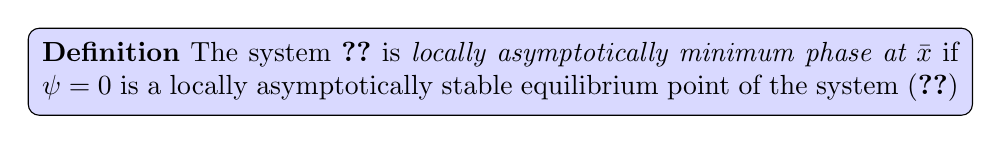
\begin{tikzpicture}
\node [mybox] (box){%
    \begin{minipage}{.96\textwidth}     %Larghezza del box
    \textbf{Definition} The system \ref{eq: system_affine} is \textit{locally asymptotically minimum phase at $\bar{x}$} if $\psi=0$ is a locally asymptotically stable equilibrium point of the system (\ref{eq: zero_dyn})
     \end{minipage}
};
\end{tikzpicture}%

\subsection{First control problem: Regulation}
In the introduction, we have seen that the most common problem in the field of automatic control are: regulation and tracking.\\
In order to obtain a \textbf{regulation} of the system (\ref{eq: system_affine}) is sufficient to define the control law:
\begin{equation}\label{eq:regulation}
    \begin{aligned}
        &u=\frac{1}{L_gL_f^{\gamma-1}h(x)u}(-L_gh(x)+v) &\text{feedback linearization}\\
        &v=-K\mu &{\color{red}{\text{linear control}}}
    \end{aligned}
\end{equation}
where $K=[k_1,..., k_\gamma]\in\mathbb{R}^\gamma$ is such that $A-BK$ is asymptotically stable. \\

\hspace*{-5mm}
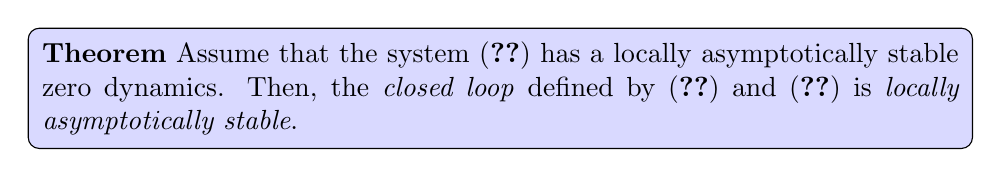
\begin{tikzpicture}
\node [mybox] (box){%
    \begin{minipage}{.96\textwidth}     %Larghezza del box
    \textbf{Theorem} Assume that the system (\ref{eq: system_affine}) has a locally asymptotically stable zero dynamics. Then, the \textit{closed loop} defined by (\ref{eq: system_affine}) and (\ref{eq:regulation}) is \textit{locally asymptotically stable}.
    \end{minipage}
};
\end{tikzpicture}%
\subsection{Second control problem: Tracking}
Now let consider the problem that the system output is required to track a desired signal $r(t)$, this signal has to be \textbf{smooth} and \textbf{bounded}. Let $\mu_r\doteq(r,\dot{r},..., r^{\gamma-1})$, we define the \textbf{tracking error} as
$$\Tilde{\mu}\doteq\mu_r-\mu$$
We would like to make this error small and possibly to force it to converge to zero. Even in this case we define: 
\begin{equation}\label{eq:tracking}
    \begin{aligned}
        &u=\frac{1}{L_gL_f^{\gamma-1}h(x)u}(-L_gh(x)+v) &\text{feedback linearization}\\
        &v=-K\Tilde{\mu}+r^{(\gamma)} &\text{linear control}
    \end{aligned}
\end{equation}
where $K=[k_1,..., k_\gamma]\in\mathbb{R}^\gamma$ is such that $A-BK$ is asymptotically stable. \\

\hspace*{-5mm}
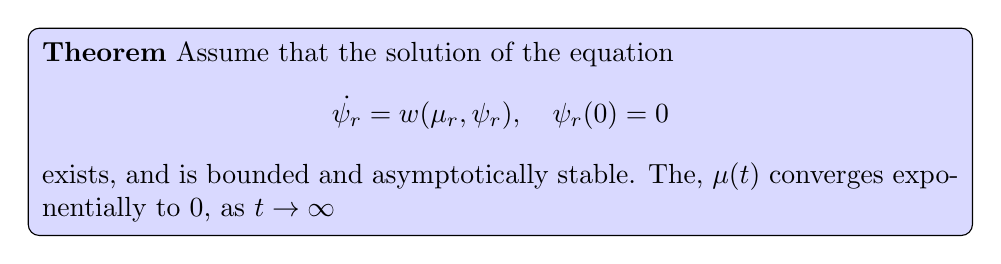
\begin{tikzpicture}
\node [mybox] (box){%
    \begin{minipage}{.96\textwidth}     %Larghezza del box
    \textbf{Theorem} Assume that the solution of the equation 
    $$\dot{\psi_r}=w(\mu_r, \psi_r), \quad \psi_r(0)=0$$
    exists, and is bounded and asymptotically stable. The, $\Tilde{\mu}(t)$ converges exponentially  to 0, as $t \rightarrow \infty$
    \end{minipage}
};
\end{tikzpicture}%

\subsection{Control scheme}
The aim of this section is to give a general control scheme for physical systems/plants controlled by using the \textit{feedback linearization}.  

\begin{figure}[h]
    \centering
    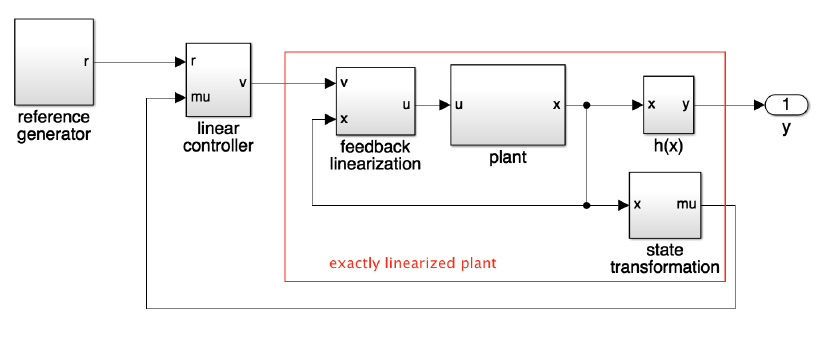
\includegraphics[scale=0.7]{NonLinearControl/images/FL_ControlScheme .png}
    \caption{Feedback linearization control scheme}
    \label{fig:FL_controlscheme}
\end{figure}

Now we are going to describe the blocks of the figure (\ref{fig:FL_controlscheme}):
\begin{itemize}
    \item \textbf{Plant}: is a nonlinear system affine in the input u of the form $\dot{x}=f(x)+g(x)u$;
    \item \textbf{State transformation}: is obtained by applying $\mu=(y, \dot{y}, ..., y^{(\gamma-1)})=(h(x), L_fh(x), ..., L_f^{\gamma-1}h(x))$
    \item \textbf{Feedback linearization}: is obtained implementing the equation \ref{eq:tracking}; 
    \item The \textbf{linear controller} can be implemented by using any technique (eg. pole placement)
\end{itemize}

\section{Discussion}
It is useful pay attention that:
\begin{enumerate}
    \item The results which has been found for Feedback linearization hold in \textit{some region} of the state space $\Omega\subseteq\mathbb{R}^n$, in particular where the multiplicative term $L_gL_f^{\gamma-1}h(x)$ is non-zero. Global results are available but we have to do stronger assumptions.
    \item We have seen that there are relevant differences with respect to \textbf{Conventional linearization}: in FL the linearization is exact on the whole region $\Omega$. Even in the case the CL worked, the Feedback linearization gives better results; 
    \item The Feedback linearization technique does not take into account problems related to the uncertainty of the nominal plant and parameters: issue linked to the robustness are provided instead by other techniques like \textit{sliding mode control}.
\end{enumerate}

\chapter{Method(2): Sliding mode control}
\textbf{Sliding mode control (SMC)} is a well-estabilished method for control of nonlinear systems, and is characterized (like Feedback linearization) by solid theoretical foundations. An interesting feature of SMC is the robustness against \textbf{imprecise knowledge of the plant to control}. \\
\textbf{General Approach}:
\begin{enumerate}
    \item A \textbf{sliding surface} is defined. This surface is a subset of the state domain where the system can have \textbf{good properties}.
    \item A feedback law is designed in order to bring the plant trajectory towards the sliding surface and once there, to stay close to this surface. 
\end{enumerate}

The SMC control law is similar to the FL control law, but the approaches are quite different. \\
In the case of control by using Feedback linearization of \textbf{Chua circuit} we have seen that the nonlinear resistor $\rho({x_1})$ brings the system to have a chaotic behaviour. Although to design the controller we have used a \textit{smooth approximation} of the nonlinearity that prevent us to use a piece-wise function which is not differentiable. If we try to apply the control to the real plant, we can see that the tracking error is very large. This is due to the fact the FL does not take into account uncertainties or approximations of the plant. We will see at the end of this chapter that the tracking error of the controlled system after that a Sliding mode controller has been applied is insignificant with respect to the Feedback linearization one. In the figure below we can note this fact: 

\begin{figure}[h]
    \centering
    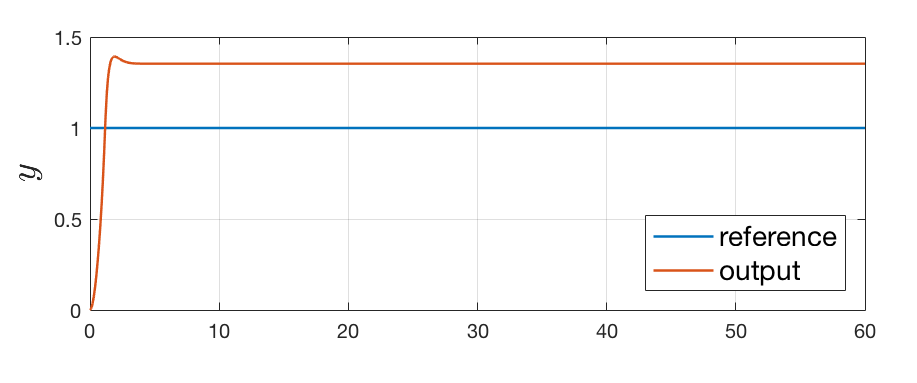
\includegraphics[scale=0.7]{NonLinearControl/images/FL_tracking.png}
    \caption{Tracking error in presence of uncertainties (FL)}
    \label{fig:enter-label}
\end{figure}

\noindent
We have the same setting as Feedback linearization, the (nonlinear) system is in the form: 
\begin{equation}
    \begin{aligned}
        &\dot{x}=f(x)+g(x)u\\
        &y=h(x)
    \end{aligned}
\end{equation}
which can be lead to the \textit{normal form} that distinguishes: the external dynamics described by the state transformation $x\rightarrow \mu$ and the internal dynamics described by $\dot{\psi}$ assumed to be locally asymptotically stable.\\
Suppose now that the system output $y(t)$ is required to track a reference signal $r(t)$. In a way similar to the FL, we define the \textit{tracking error} as $\Tilde{y}\doteq  r-y$. Even in this case we want to make it "small" and force it to converge to zero.\\

Now a set of definitions are given as ingredient to introduce the \textbf{Sliding mode control} method.\\

\hspace*{-5mm}
\begin{tikzpicture}
\node [mybox] (box){%
    \begin{minipage}{.96\textwidth}     %Larghezza del box
    \textbf{Definition (Sliding surface)} The \textbf{sliding surface} is $$S(t)\doteq\{x\in \mathbb{R}^n : \textbf{s}(x, t)=0 \}$$ where the function $\textbf{s}:\mathbb{R}^{n+1}\rightarrow\mathbb{R}$ is defined as follows
    \begin{align*}
        \textbf{s}(x,t)&=\Tilde{y}^{(\gamma-1)}+k_\gamma \Tilde{y}^{(\gamma-2)}+...+k_2\Tilde{y}=\\
        &=\Tilde{\mu}_\gamma+k_\gamma \ \Tilde{\mu}_{\gamma-1}+...+k_2 \ \Tilde{\mu}_1   
    \end{align*}
    
    the coefficients $k_i\in \mathbb{R}$ are chosen so that the roots of the polynomial ${P(\lambda)=\lambda^{\gamma-1}+k_\gamma\lambda^{\gamma-2}+...+k_2}$ have \textbf{negative real part}.
    \end{minipage}
};
\end{tikzpicture}%

\section{Behaviour on the sliding surface}
{\color{red} \textbf{Property 1}}: If the trajectory of the system is confined to the sliding surface, then the tracking error $\Tilde{y}\rightarrow 0$, in a way that depends on the root of $P(\lambda)$.\\

Due to the fact that the system has a nice behaviour if the \textbf{Property 1} is verified, we would like to find a control law such that the sliding surface $S$ could be: 
\begin{itemize}
    \item \textbf{\underline{Invariant}}: if the trajectory is on S, it remains on it; that is $x(\tau)\in S(\tau) \Rightarrow x(t)\in S(t), \forall t \ge \tau$; 
    \item \textbf{\underline{Attractive}}: if the trajectory is outside of the sliding surface $S$, it is forced to move toward it in a finite time.
\end{itemize}

The motion of the system on this surface is called \textbf{sliding mode}, from this fact is derived the name \textbf{Sliding mode control}.

\begin{figure}[h]
    \centering
    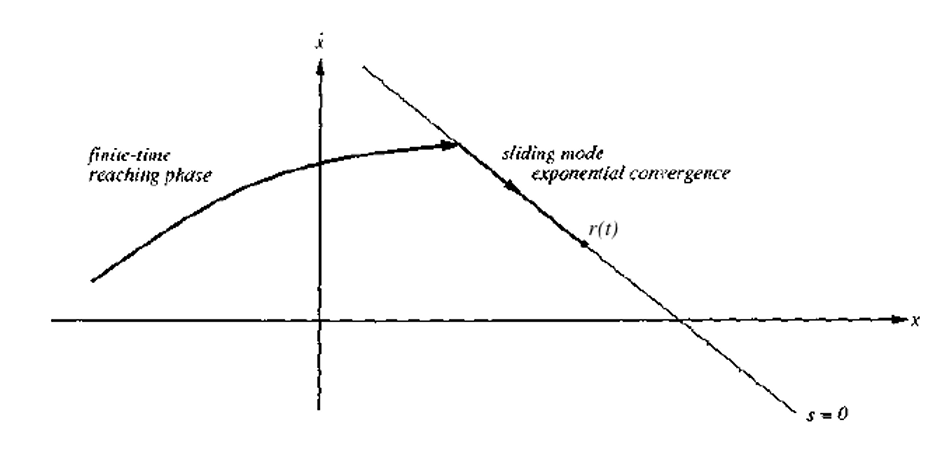
\includegraphics[scale=0.7]{NonLinearControl/images/SMC.png}
    \label{fig:enter-label}
\end{figure}

\subsection{Invariance of the Sliding surface}
If in a certain time $\tau$ the trajectory of the system lie on the sliding surface, then as defined before $x(\tau)\in S \Rightarrow \textbf{s}(x(\tau), \tau)=0$. In order to guarantee the invariance of the surface we have to put $\dot{\textbf{s}}=0 \quad \forall t$.\\
\begin{align*}
&\dot{\textbf{s}}=\Tilde{y}^{(\gamma)}+k_\gamma \Tilde{y}^{(\gamma-1)}+...+k_2\dot{\Tilde{y}}=0 \Longleftrightarrow r^{(\gamma)}-a(x)-b(x)u+k_\gamma y^{(\gamma-1)}+...+k_2 \dot{\Tilde{y}}=0\\
    &
\end{align*}
where we used $\Tilde{y}^{(\gamma)}=r^{(\gamma)}-y^{(\gamma)}=
r^{(\gamma)}-a(x)-b(x)u$. \\
Solving the equation for $u$ we obtain the following control law
\begin{equation}
    u_s=\frac{1}{b(x)}\bigg(r^{(\gamma)}-a(x)+k_\gamma \Tilde{y}^{(\gamma-1)}+...+k_2 \dot{\Tilde{y}} \bigg)
\end{equation}
\noindent
{\color{red} \textbf{Property 2}}: using this law, the sliding surface is an \underline{invariant set}. 

\subsection{Attractiveness of the Sliding surface}
Suppose that at a certain instant $\tau$ the trajectory is not on the sliding surface. We would like to bring it toward $S(t)$ in a finite time. \\
The introduction of a discontinuous term to $u_s$ make $S$ attractive. Then, the \textit{complete control law} is the following, let $k_1>0$: 
$$ u_s=\frac{1}{b(x)}\bigg(r^{(\gamma)}-a(x)+k_\gamma \Tilde{y}^{(\gamma-1)}+...+k_2 \dot{\Tilde{y}} +k_1 \text{sign}(\textbf{s}(x,t))\bigg)$$
The motivation of adding a discontinuous term is the fact that in this way the derivative of the sliding function 
\begin{align}
    \dot{\textbf{s}}(x,t)&= r^{(\gamma)}-a(x)-b(x)u+k_\gamma \Tilde{y}^{(\gamma-1)}+...+k_2 \dot{\Tilde{y}}=\\
    &=-k_1\text{sign}(\textbf{s}(x,t)).
\end{align}

\noindent
{\color{red}\textbf{Property 3}}:  $\textbf{s}(x,t) \ \dot{\textbf{s}}(x,t)<0,\quad \forall x,t$, which implies that $S(t)$ is attractive (the sliding function \textbf{s} converges to zero in finite time). In particular: 
\begin{itemize}
    \item $\textbf{s}(x,\tau)>0 \Rightarrow \dot{\textbf{s}}=-k_1 $
    \begin{align*}
        &\int_{\tau}^{t} \dot{\textbf{s}}\ dt = \int_{\tau}^{t} -k_1\ dt 
        \Longleftrightarrow \textbf{s}(t)-\textbf{s}(\tau)=-k_1(t-\tau) \Longleftrightarrow
        &\textbf{s}(t)=\textbf{s}(\tau)-k_1(t-\tau)
    \end{align*}
    \item $\textbf{s}(x,\tau)<0 \Rightarrow \dot{\textbf{s}}=k_1$
    \begin{align*}
       &\int_{\tau}^{t} \dot{\textbf{s}}\ dt = \int_{\tau}^{t} k_1\ dt 
        \Longleftrightarrow \textbf{s}(t)-\textbf{s}(\tau)=k_1(t-\tau) \Longleftrightarrow
        &\textbf{s}(t)=\textbf{s}(\tau)+k_1(t-\tau)
    \end{align*}
\end{itemize}

\noindent
In both cases, $\textbf{s}(t)\rightarrow 0$ in finite time $\Rightarrow$ $x(t)\rightarrow S(t)$ in finite time applying the input with discontinuous term.

\subsection{Chattering}
The presence of the discontinuous term may cause a phenomenon called \textbf{chattering} which consists of high frequency oscillations around the sliding surface. To avoid this problem we can use a \textbf{sigmoid function} $\sigma(\eta \textbf{s})$, where $\eta$ is a design parameter which defines the slope of the sigmoid itself. The function $\sigma(\eta\textbf{s})=\tanh{(\eta\textbf{s})}$ is a typical choice. The control law becomes:\\

\begin{figure}[h]
    \centering
    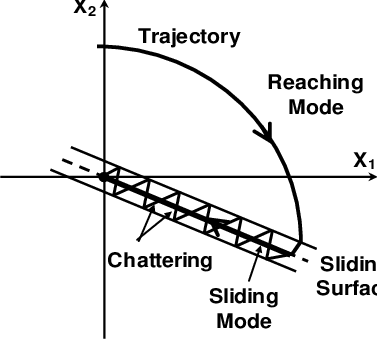
\includegraphics[scale=0.7]{NonLinearControl/images/Chattering.png}
    \caption{Chattering phenomenon}
    \label{fig:enter-label}
\end{figure}

\hspace*{-5mm}
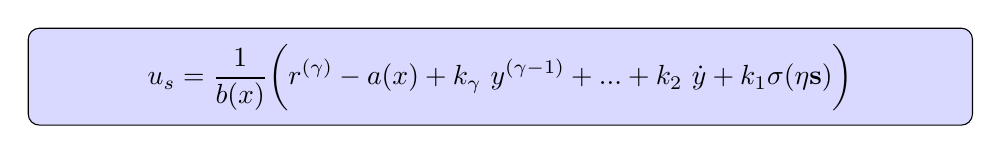
\begin{tikzpicture}
\node [mybox] (box){%
    \begin{minipage}{.96\textwidth}     %Larghezza del box
    $$u_s=\frac{1}{b(x)}\bigg(r^{(\gamma)}-a(x)+k_\gamma \ \Tilde{y}^{(\gamma-1)}+...+k_2 \ \dot{\Tilde{y}} +k_1 \sigma(\eta\textbf{s})\bigg) $$
    \end{minipage}
};
\end{tikzpicture}%
\begin{figure}[h]
    \centering
    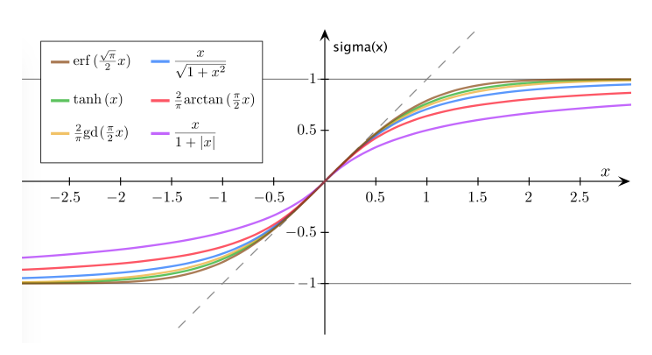
\includegraphics{NonLinearControl/images/sigmoids.png}
    \caption{Alternatives to sign(\textbf{s})}
    \label{fig:enter-label}
\end{figure}

\section{Comparison with feedback linearization}
The two approaches of \textbf{Feedback linearization} and \textbf{Sliding mode control} have a common general control law given by: 
$$u=\frac{1}{L_gL_f^{\gamma-1}h(x)}(-L_f^{\gamma}h(x)+v)=\frac{1}{b(x)}(-a(x)+v)$$
The techniques have the $v$ which differs of a term. More specifically, let $\Tilde{\mu}_i=r^{(i)}-y^{(i)}=\tilde{y}^{(i)}$
\begin{itemize}
    \item In the feedback linearization: $v=r^{(\gamma)}+k_\gamma \ \Tilde{\mu}_\gamma+...+k_1 \ \Tilde{\mu}_1$
    \item In the sliding mode control: $v=r^{(\gamma)}+k_\gamma \ \Tilde{\mu}_\gamma+...+k_1 \ \sigma(\eta\textbf{s})$
\end{itemize}
The term which is different increases the robustness of the controller.

\section{Control Scheme}
Even the general control scheme is quite similar to the feedback linearization, the only difference is that instead of the linear controller there is a block that provided $r^{(\gamma)}$ and $\Tilde{\mu}$ gives the sliding control law $v=r^{(\gamma)}+k_\gamma \ \Tilde{\mu}_\gamma+...+k_1 \ \sigma(\eta\textbf{s})$

\begin{figure}[h]
    \centering
    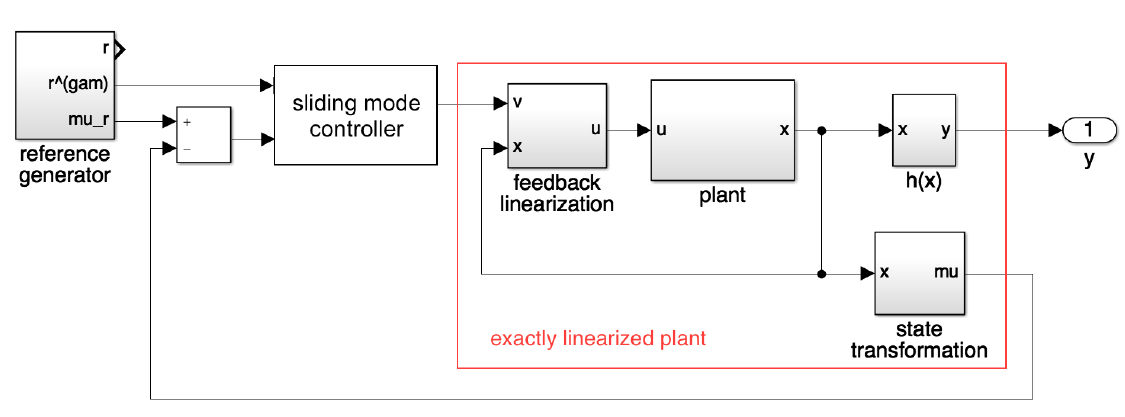
\includegraphics[scale=0.6]{NonLinearControl/images/SMC_ControlScheme.png}
    \caption{Sliding control mode general control scheme}
    \label{fig:enter-label}
\end{figure}



\section{Robustness properties}
Now we consider the case when the system to control in \underline{not exactly known}. In normal form we can describe the fact in this way: 
{\color{red}$$y^{(\gamma)}=a(x)+\Delta a(x) +b(x)u$$}

Where $\Delta a(x)$ is a smooth function of $\mathbb{R}^{n_x}$ but it is \underline{unknown}, moreover we know that ${\lVert \Delta a(x) \rVert \le \bar{\Delta}, \ \forall x \in \mathbb{R}^n}$. In this way the time derivative of the sliding function is: 
$$ \dot{\textbf{s}}(x, t)=-\Delta a(x)-k_1 \ \sigma(\eta\textbf{s})$$
In the context of uncertainty in the model of the plant it holds that:\\

\noindent
{\color{red}\textbf{Property 4}}: If $k_1>\bar{\Delta}$, then the sliding surface is attractive. \\

The figure below shows the \textit{step response} for a sliding mode controlled system in which uncertainty appears. In particular for control design we use the approximated $\hat{\rho}(x_1)$, while the plant has the real nonlinearity which is a piece-wise function $\rho(x_1)$. The tracking error is smaller than the case of a controller built by using the feedback linearization technique.

\begin{figure}[h]
    \centering
    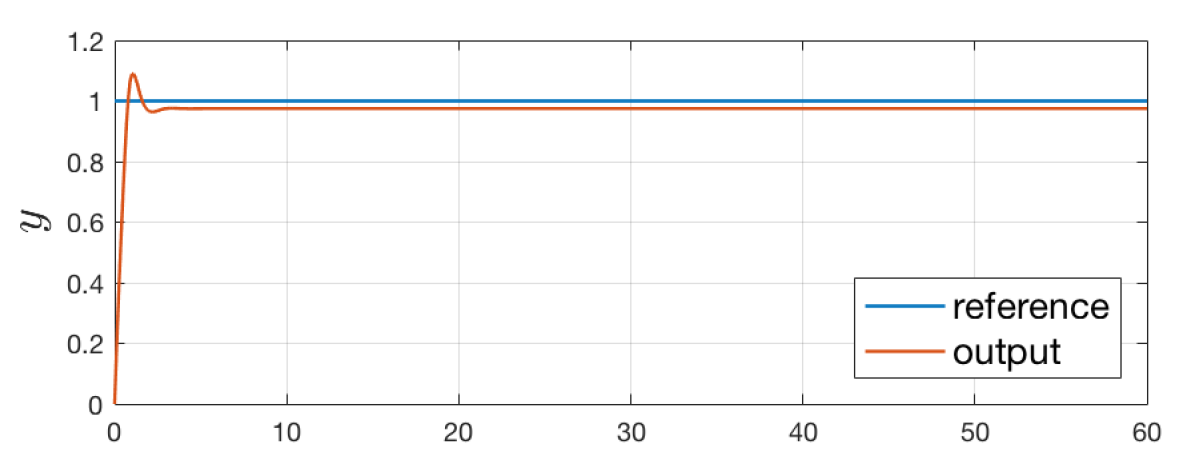
\includegraphics[scale=0.7]{NonLinearControl/images/SMC_Tracking.png}
    \caption{Step response: sliding mode controller}
    \label{fig:enter-label}
\end{figure}

\section{Guidelines for the choice of the SM parameters}
\begin{itemize}
    \item The parameters $k_i, \ i=\gamma, \gamma-1, ..., 2$ are the coefficients  of the polynomial $P(\lambda)$. Useful indications can be:
    \begin{itemize}
        \item All the roots must have negative real part;
        \item The speed of convergence is linked to the value of the $k_i$
        \item At the same time they cannot be too much large this would result in too high command activity
    \end{itemize}
    \item The parameter $k_1>0$ allows us to \textbf{increase the closed-loop robustness}: The larger is $k_1$ the more robust is the closed-loop system, but too large value of this parameter results in significant \textbf{chattering phenomena} and \textbf{high command activity};
    \item Using the hyperbolic tangent function instead of sign requires to choose the additional parameter $\eta$. A large value of $\eta$ can be taken initially so that $\tanh \simeq \text{sign}$, then $\eta$ can be gradually reduced in order to reduce the chattering pheonomena without compromising too much \textbf{performance} and \textbf{robustness}.
    
\end{itemize}

\section{Discussion}
Sliding mode control is a technique which has strong theoretical behaviuor, is robust to model uncertainties and disturbances of a certain type for the mentioned reasons this method give \textbf{high control performances}. \\
On the other hand, as usual, there are some \textbf{drawbacks}:
\begin{itemize}
    \item The model is assumed to be affine in $u$, it cannot have whatever structure; 
    \item When the internal dynamics is stable everything works well, otherwise we can't approach the control problem; sometimes it is sufficient to change the output to make the same problem easier and so tractable; 
    \item in general there is an \textbf{high command activity}.
\end{itemize}
Possible extensions of the concepts exposed here are possible for systems which have multiple input and multiple output (MIMO).


\chapter{Method(4): Non linear Model predictive control (NMPC)}
In this chapter it will be illustrated a technique of control called \textbf{Nonlinear Model Predictive Control}. Other techniques we treated did not need some specific math tools in order to be explained and understood. This time we need some instruments that guide us to the study of this powerful and general control method.

\section{Math tools}
\subsection{Vector and signal norms}

{\color{blue} \subsubsection{Vector spaces}
}
\subsubsection{Vector spaces}
A \textbf{linear vector space } $F$ over a field $\mathbb{A}$ is a \textit{set} equipped of two operations: 
\begin{enumerate}
    \item \textbf{Vector addition}: $\forall f, g \ \in F \Leftarrow f+g\in F$
    \item \textbf{Scalar multiplication}: $\forall \alpha\in \mathbb{R}, \ f \in F \Leftarrow \alpha f \in F$
\end{enumerate}
Let us put together these two properties obtaining: 
{
\large{
    \begin{equation*}
    \forall \alpha, \beta \in \mathbb{R}, \ \forall f, g \in F \leftarrow 
    \alpha f + \beta g \in F
\end{equation*}
}
}
{\color{blue} \subsubsection{Norm: general definition} }

A \textbf{norm} is a function $\lVert  \diamond \rVert : \mathbb{R}^n\rightarrow\mathbb{R}$ which satisfies the following properties: 
\begin{enumerate}
    \item $\lVert x \rVert \ge 0$
    \item $ \Vert \alpha x \rVert = \alpha \lVert x \rVert$
    \item $\lVert x+y \rVert \le \lVert x \rVert + \lVert y \rVert $ (triangular inequality)
    \item $\lVert x \rVert=0 \Longleftrightarrow x=0$
\end{enumerate}
{\color{blue} \subsubsection{Vector norm}}

Let us consider a vector $f=(f_1, ..., f_n)^T\in\mathbb{R}^n$, we can define some norm functions in particular $\ell_1, \ell_2$ and $\ell_\infty$ norms:
\begin{itemize}
    \item \underline{$\ell_1$-norm} is defined as: $\lVert f \rVert_1=\sum_{i=1}^{n}\lvert f_i \rvert$ 
    \item \underline{$\ell_2$-norm} is defined as: 
    $\lVert f \rVert_2=\sqrt{\sum_{i=1}^n f_i^2}$
    \item \underline{$\ell_\infty$-norm} is defined as:
   $ \lVert f \rVert_\infty=\max_{i=1,..., n} \lvert f_i \rvert$
    \item \underline{$\ell_2$ weighted norm} is defined as: 
    $\lVert f \rVert_{Q,2}=\sqrt{f^T Q f}=\sqrt{\sum_{i=1}^n qi f_i^2}$
\end{itemize}
The last type of norm is used when one want to give more or less importance to a certain component in the vector.

{\color{red}In \textsc{Matlab}} the command in order to compute a norm of a vector $f$ properly defined is \texttt{norm(f)}, by default it is the $\ell_2$-norm if not specified, otherwise one should use the commands \texttt{norm(f,1)} to indicate the $\ell_1$-norm and \texttt{norm(f,inf)} in order to indicate the $\ell_\infty$-norm. \\
{\color{blue} \subsubsection{Signal norm}}

Another important type of norm is that of a \textbf{signal} which is defined in a similar way with respect to the vector case. We consider both the cases of \textit{scalar function} and \textit{vector valued} functions. The main difference wrt the vectors is the fact that we have integrals instead of summations, a function can be seen as a vector composed by an \textbf{infinite number of elements}. \\

\noindent
\textbf{First case: $f: \mathbb{R}\to \mathbb{R}$}.
We have the following definitions: 
\begin{align}
    &\Vert f(t) \Vert_1 = \int_{0}^{\infty} {\vert f(t) \vert \ dt} \quad (L_1-\text{norm})\\
    &\Vert f(t) \Vert_2 = \int_{0}^{\infty} {[f(t)]^2 \ dt} \quad (L_2-\text{norm})\\
    &\Vert f(t) \Vert_\infty =  \sup_{t\in\mathbb{R}^+} \vert f(t) \vert \quad (L_\infty-\text{norm}) \label{eq:f_inf}
\end{align}
{\color{red}In \textsc{Matlab}} it is a little bit more complicated to compute a norm of a function because at first we cannot treat infinite values with the computer. A way to overcome this fact is to define a variable \texttt{dt} as a \textit{sample step} and evaluate the function in a large number of points, then we can approximately calculate the norm by using the 'standard' command \texttt{norm}.
Then, we have for example: 
{\color{blue}
\begin{verbatim}
    dt=0.0001;
    t=linspace(0,100, dt); 
    f=sin(t); 

    L2   = norm(f,2)*sqrt(dt);       %L_2 norm
    L1   = norm(f,1)*dt;             %L_1 norm
    Linf = norm(f,inf);              %L_inf norm          
\end{verbatim}
}

The multiplicative terms \texttt{sqrt(dt)} and \texttt{dt} are been added in order to apply the definition. By doing the above calculations we have approximated the integrals.\\


\noindent
\textbf{Second case: $f:\mathbb{R}\to\mathbb{R}^n$}. This is the case of \textbf{vector-valued} functions in which $\forall t \in \mathbb{R}^+$ we have a vector $f(t)\in\mathbb{R}^n$. The definitions previously given are modified as follows (basically we have norms instead of absolute values due to the fact that for each $t$, you have a vector instead of a scalar): 
\begin{align}
    &\Vert f(t) \Vert_1 = \int_{0}^{\infty} \Vert f(t) \Vert_1 \ dt \quad (L_1-\text{norm})\\
    &\Vert f(t) \Vert_2 = \sqrt{\int_{0}^{\infty} \Vert f(t) \Vert_2^2 \ dt}=
    \sqrt{\int_{0}^{\infty} f(t)^Tf(t) \ dt } \quad (L_2-\text{norm})\\
    &\Vert f(t) \Vert_2 = \sup_{t\in\mathbb{R}^+} \Vert f(t) \Vert_\infty \quad (L_\infty-\text{norm}) \label{eq: fv_inf}\\ 
    &\Vert f(t) \Vert_{Q,2} = \sqrt{\int_{0}^{\infty} f(t)^T \ Q \ f(t) \ dt }  \quad (L_1 \  \text{weighted norm})
\end{align}
An observation can be done on (\ref{eq:f_inf}) and (\ref{eq: fv_inf}): the $\sup$ generalizes the concept of maximum, in particular a function might not assume the value of the maximum. \\
{\color{red}In \textsc{Matlab}} the \textbf{weighted $\ell_2$-norm} can be computed as follows:

{\color{blue}
\begin{verbatim}
    dt=0.0001; 
    t=linspace(0,100, dt);  
    f=[exp(-3*t); sin(3*t)];        %vector valued function 
    Q=diag(1,2,3); 
    
    L2 = sqrt( sum ( sum (Q*f.^2) * dt ) );
    %           ^     ^
    %           |     |
    %         \int   l2-norm
\end{verbatim}

}


\subsection{Optimization}
\textbf{Optimization} is a branch of Maths that deals with \textbf{finding the best solution to a problem} which is \textit{finding the minimum} of a function. Optimization acts a fundamental role in many engineering field and also in \textbf{control design} is important: when we design a controller we want to: (i) minimize the tracking error; (ii) minimize the command effort as the actuators has got limited working ranges; (iii) minimize the effect of disturbances. In our case we introduce it, in order to apply it to \textit{Model Predictive Control}.

{\color{blue}\subsubsection{Basic notions}}
In the \textbf{univariate function} $f: \mathbb{R}\to\mathbb{R}$ the problem of minimization is the following: 
{\large{

\begin{align}
   &x^*=\text{arg}\min_{x\in\mathbb{R}} f(x) \label{eq:minimizer}\\
    &f(x^*)=\min_{x\in\mathbb{R}} f(x) \label{eq: minimum}
\end{align}

}}

The (\ref{eq:minimizer}) is called the \textbf{minizer} while the (\ref{eq: minimum}) is called the \textbf{minimum}. The $x$ is the \textbf{decision variable}, while $f(\diamond)$ is called either the \textbf{objective function} or \textbf{cost function} or \textbf{loss function} (used in AI).\\
In a univariate problem there could be: \textit{one global minimum}, \textit{several global minima}, \textit{infinite global minima}. The optimization problems usually require that the solution (minimizer) observes some \textbf{constraints}, in this case we are talking about \textbf{constrained minimization}. As the constraints could be more than one, an alternative notation for the problem (\ref{eq:minimizer}) is:

{\large{
\begin{equation}
    \begin{aligned}
        \min \ &f(x)\\
        &\text{subject to} \ x\in \mathbb{R}
    \end{aligned}
\end{equation}

}}

Where \textit{subject to} is often abbreviated as \textbf{s.t.}\\
In order to start talking about optimization we considered the \textbf{univariate} case in which the decision is taken according a \textbf{single variable}, in engineering problems the decision variable can be hundreds or thousands! The graphical representation becomes not possible at all, but the concepts we exposed previously remain more or less the same but more general. We are talking about in this case of \textbf{multivariate functions}. In particular: 
\begin{itemize}
    \item The \textbf{objective function} $f(x)$ is such that $f:\mathbb{R}^n\to\mathbb{R}$
    \item The \textbf{decision variable} is a vector $x\in\mathbb{R}^n$
    \item Also the \textbf{minimizer} is a vector $x^*\in \mathbb{R}^n$
\end{itemize}
An Optimization problem is said to be \textbf{feasible} if there is at least a solution, otherwise it is said to be \textbf{unfeasible}. We can define in this way a \textbf{feasible set} as:
{\large{

\begin{equation}
    \mathcal{X}^*=\{x^* \in \mathbb{R}^n \ : p=f(x^*) \}
\end{equation}
}}

where $p$ is the minimum. We can immediately understand that when an optimization problem is \textit{unfeasible} is such that $\mathcal{X}^*=\emptyset$. \\
Surely a nice class of optimization problems is the \textbf{convex optimization} class.

{\color{blue} \subsubsection{Minimization}}
\noindent
In some simple cases it is possible to find an analytical solution to an optimization problems, on the other hand in the great majority of the real optimization problems it is not possible to find in a simple way an analytical solution.\\
In these cases, otherwise, a \textbf{numerical solution} can be found by using an iterative algorithm which starts at a certain point $x^O$, and based on the \textbf{gradient function}, other points are visited. There are some functions which have "nice properties", the \textbf{convex functions} their local minimum are global mimimum. It is remarkable that the \textit{level curves} of a convex function define \textbf{convex sets}.\\

\section{Introduction to NMPC}
\textbf{Nonlinear Model Predictive Control (NMPC)} is a general control methods which differently than the others that has been treated, provide us with a way for taking into account both the aspects related to: 
\begin{itemize}
    \item \textbf{Constraints} which are applied either on input, state or output; 
    \item \textbf{Trade off between performance and command activity} which is managed in a systematic way how will be seen.
\end{itemize}
The \textbf{Approach} of this control technique is the following. At each time step: 
\begin{enumerate}
    \item A prediction \textbf{over a given time horizon} is performed using a model of the plant; 
    \item The command input is chosen as the one yielding the "best" prediction, that is the closer to the specified behaviour and this is done by solving an \textbf{online optimization algorithm}
\end{enumerate}

This time the mathematical form of the plant is not assumed to be \textbf{affine} like in the Feedback linearization and Sliding Mode control, but it is in general a MIMO system characterized by
\begin{equation} \label{eq: MIMO_system}
    \begin{aligned}
        &\dot{x}=f(x,u)\\
        &y=h(x,u)
    \end{aligned}
\end{equation}
where $x, y$ and $u$ are as usual the state, the output and the input. A generalization to time varying systems could be done without particular efforts.\\
The state is measured in \textbf{real time}, with a proper sampling time $T_s$. The measurement are:
$$x(t_k), \ t_k=T_sk, \  k=0,1, ...$$
If the state cannot be measured an observer has to be employed. 

\section{First step: Prediction}
At each time $t=t_k$ both the \textbf{state} $\hat{x}(\tau)$ and the \textbf{output} $\hat{y}(\tau)$ are predicted over the time interval $[t, t+T_p]$ by integrating (\ref{eq: MIMO_system}). The time $T_p \ge T_s$ is called the \textbf{prediction horizon}. For each $\tau\in [t,t+T_p]$, the quantity $\hat{y}(\tau)$ (the \textbf{predicted output}) depends on:
\begin{itemize}
    \item The \textbf{initial state} $x(t)$
    \item The \textbf{input signal} $u(t:\tau)$ which denotes a generic input signal in the interval $[t, \tau]$, this is an \textbf{open-loop} signal in the sense that it depends on the initial state $x(t)$, but not on $x(\tau)$ that is the "current" state.
\end{itemize}

\section{Second step: Optimization}
At each time $t=t_k$ we find an \textbf{input signal} $u(t:\tau)=u^*(t:\tau)$ such that the \underline{prediction}  
$$
    \hat{y}(x(t), u^*(t:\tau))\equiv \hat{y}(u^*(t:\tau))
$$
has the \underline{desired behaviour} for all $\tau \in [t, t+T_p]$. We seek a signal that for each sub-interval $[t,\tau]$ gave the desired behaviour. This concept is formalize by defining the objective function   \\

\hspace*{-5mm}
\begin{tikzpicture}
\node [mybox] (box){%
    \begin{minipage}{.96\textwidth}     %Larghezza del box
        {\large{
        \begin{equation*}
            J(u(t:t+T_p)) = \int_{t}^{t+T_p} {(\Vert \Tilde{y}(\tau) \Vert_Q^2 + \Vert u(\tau) \Vert_R^2 )  \ d\tau} + \Vert \Tilde{y}(t + T_p) \Vert_P
        \end{equation*}
        
        }}
    \end{minipage}
};
\end{tikzpicture}%


the term $\tilde{y}(\tau)=r(\tau)-\hat{y}(\tau)$ is the \textbf{predicted tracking error}, $r(\tau)\in\mathbb{R}^{n_y}$ is a \textbf{reference to track}, while $\Vert \diamond \Vert_X$ is the \textbf{weighted norm}. The input $u^*(t:t+T_p)$ is chosen as one \textbf{minimizing} the objective function $J(u(t:t+T_p))$, in which:
\begin{itemize}
    \item The term $\Vert \tilde{y}(\tau) \Vert_Q^2$ is for minimizing the tracking error over a finite interval; 
    \item The term $\Vert \tilde{y}(t+T_p) \Vert_P^2$ gives importance to the final tracking error; 
    \item Finally the term $\Vert u(\tau) \Vert_R^2$ allows us to manage in a systematic way the performance beetween command activity and performances. 
\end{itemize}

The predicted tracking error $\tilde{y}(\tau)$ depends on the \textit{predicted output} which is derived from the integration of (\ref{eq: MIMO_system}), so the \textbf{minimization of the functional $J$} is therefore subject to the constraints:
\begin{align*}
    &\dot{\hat{x}}(\tau)=f(\hat{x}(\tau), u(\tau)), \ \hat{x}(t)=x(t), \tau\in[t, t+T_p]\\
    &\hat{y}(\tau)=h(\hat{x}(\tau), u(\tau)) 
\end{align*}
Other constraints can be present on:
\begin{itemize}
    \item The output or the state (eg. collision avoidance, obstacles) so that we have $\hat{x}(\tau) \in X_c$ and $\hat{y}(\tau)\in Y_c$; 
    \item The input (eg. input saturation) so that we have $u(\tau) \in U_c$;
\end{itemize}
The image below \textbf{summarizes} the steps of NMPC which are done for each $t=t_k$ many feasible solutions {\color{blue} $u(t:t+Tp)$} are provided, in the \textbf{prediction step}, relative predicted output and state are computed by using a model of the plant, for each of these choices I compute the quantity $J(u(t:t+T_p)$, finally in the \textbf{optimization step}, I select the best choice {\color{red} $u^*(t:t+T_p)$}. 

\begin{figure}[h]
    \centering
    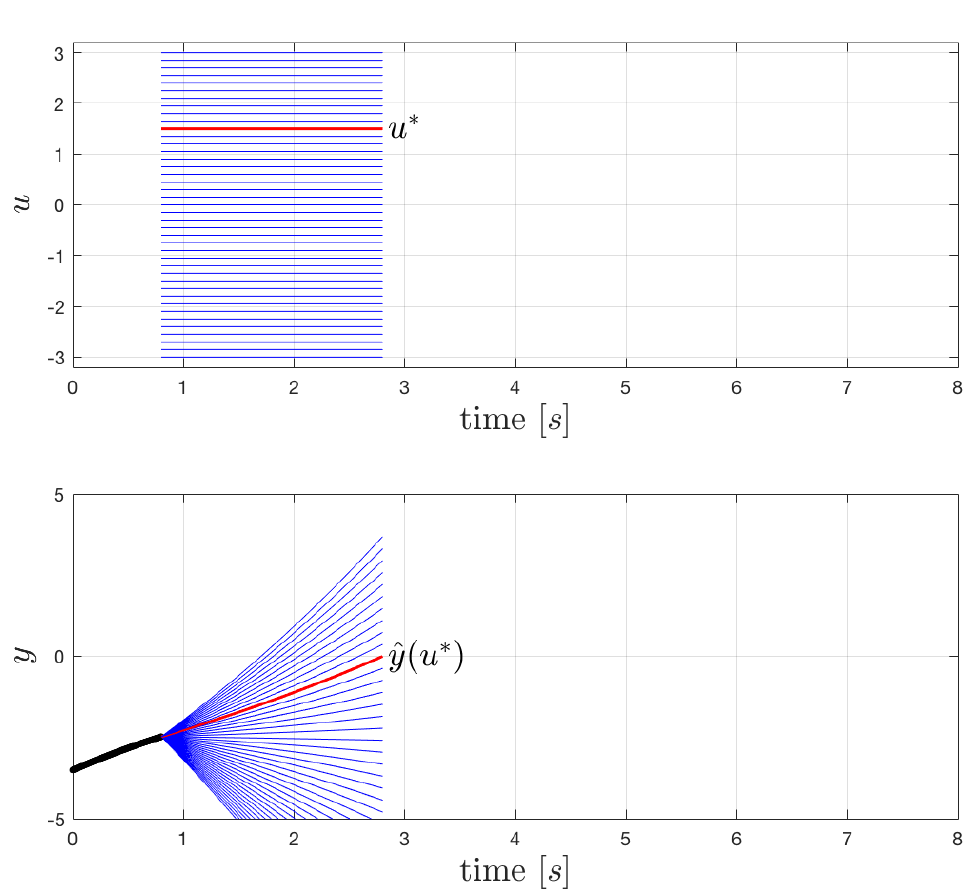
\includegraphics[scale=0.6]{NonLinearControl/images/NMPC_graph.png}
    \caption{Example of a step of Prediction and Minimization}
    \label{fig:enter-label}
\end{figure}

For each $t=t_k$ and $\tau \in [t, t+T_p]$ the following \textit{optimization problem} is solved:\\

\hspace*{-5mm}
\begin{tikzpicture}
\node [mybox] (box){%
    \begin{minipage}{.96\textwidth}     %Larghezza del box
    {\large{
\begin{equation} \label{eq:opt_alg}
    \begin{aligned}
        &u^*(t:t+T_p)=\text{arg}\min_{u(\cdot)} J(u(t:t+T_p)\\
        &\text{subject to:}\\
        &\dot{\hat{x}}(\tau)=f(\hat{x}(\tau), u(\tau)), \ \hat{x}(t)=x(t)  \quad (\text{\small{initial conditions)}}\\
        &\hat{y}(\tau)=h(\hat{x}(\tau), u(\tau)) \\
        &\hat{x}(\tau) \in \mathcal{X}_c, \ \hat{y}(\tau)\in \mathcal{Y}_c, \ u(\tau) \in \mathcal{U}_c
    \end{aligned}   
\end{equation}
}}
    \end{minipage}
};
\end{tikzpicture}%


where $T_s$  is the sampling time, $T_p\ge T_s$ is the \textbf{prediction horizon}. The exposed optimization problem is in general \textbf{non-convex} moreover must be solved online. Usually such optimization problem is solved by using efficient numerical algorithms. 

\section{Reciding Horizon}
Suppose that at a certain time $t=t_k$, the problem (\ref{eq:opt_alg}) is solved and a $u^*
(t:t+T_p)$ is found, as we mentioned this is an open-loop input,in fact it depends on $x(t)$, but not on $x(\tau), \tau>t$. For this reason If we applied this input in the whole interval $[t, t+T_p]$, we would not have be able to \textbf{increase the precision} or \textbf{adapt to a varying scenario}. At this point the \textbf{NMPC feedback control algorithm} is obtained applying the so-called \textit{receding horizon strategy}:\\

\hspace*{-5mm}
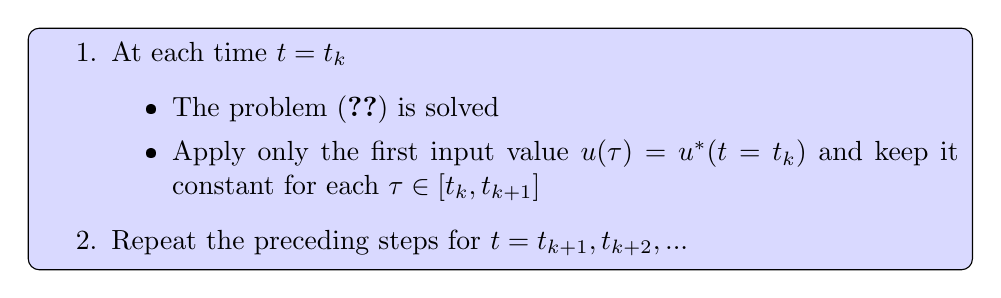
\begin{tikzpicture}
\node [mybox] (box){%
    \begin{minipage}{.96\textwidth}     %Larghezza del box
        \begin{enumerate}
            \item At each time $t=t_k$
            \begin{itemize}
                \item The problem (\ref{eq:opt_alg}) is solved
                \item Apply only the first input value $u(\tau)=u^*(t=t_k)$ and keep it constant for each $\tau \in [t_k, t_{k+1}]$
            \end{itemize}
            \item Repeat the preceding steps for  $t=t_{k+1}, t_{k+2},...$
        \end{enumerate}
    \end{minipage}
};
\end{tikzpicture}%


 
\section{Closed-loop scheme}
As it has been done in the explanation of the previous techniques of Nonlinear control, now we show the control scheme for a plant controlled by using the NMPC technique. 
The \textbf{plant} is in the form (\ref{eq: MIMO_system}), the block \textbf{NMPC} contains an on-line algorithm which solve the optimization problem and apply the \textit{reciding horizon strategy}.

\begin{figure}[h]
    \centering
    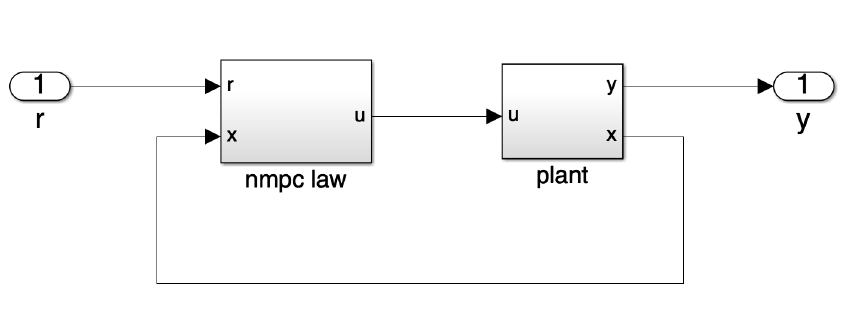
\includegraphics[scale=0.7]{NonLinearControl/images/NMPC_CtrlScheme.png}
    \caption{Control Scheme for NMPC}
    \label{fig:NMPC_ctrl}
\end{figure}

\section{NMPC design}

\subsection{Choice of the parameters}
\begin{itemize}
    \item $\mathbf{T_s}$, sufficiently small in order to respect the Nyquist-Shannon Theorem, but not too small this would result in slow computation; sometimes cannot be chosen.
    \item $\mathbf{T_p}$ it is determined through a trial and error procedure in simulation keeping in mind that a "large" $T_p$ increases the \textbf{closed-loop stability}, a "too large" $T_p$ would result in reducing in the \textbf{short-time tracking accuracy}.
\end{itemize}

\subsection{Choice of the weight matrices}
The \textbf{initial choice} of the \textbf{weight matrices} $Q, R, P$ can be diagonal non negative  such that \\

\hspace*{-5mm}
\begin{tikzpicture}
\node [mybox] (box){%
    \begin{minipage}{.96\textwidth}     %Larghezza del box
        \begin{align*}
    &Q_{ii}=\begin{cases}
        >0 & \text{in the presence of requirements  on} y_i\\
        =0  & \text{otherwise}
    \end{cases}\\
     &R_{ii}=\begin{cases}
        >0 & \text{in the presence of requirements  on} u_i\\
        =0  & \text{otherwise}
    \end{cases}\\
     &P_{ii}=\begin{cases}
        >0 & \text{in the presence of requirements  on} y_i\\
        =0  & \text{otherwise}
    \end{cases}
\end{align*}
    \end{minipage}
};
\end{tikzpicture}%


The weight matrices can be tuned by \textbf{trial/error procedure} considering that: 
\begin{itemize}
    \item Increasing $Q_{ii}, P_{ii} \Rightarrow$ decreasing of the energy of $x_i, y_i \Rightarrow$ reducing \textbf{oscillations} and \textbf{convergence time}; 
    \item Increasing $R_{ii} \Leftarrow$ decreasing of the energy of $u_i \Leftarrow$ reducing \textbf{command effort} and \textbf{energy consumption}. 
\end{itemize}

\section{Discussion}
Through our discussion we have mentioned yet, which are the advantages and disadvantages of such type of approach. But it is not bad repeat them: 
\begin{itemize}
    \item[+] NMPC is a general and flexible methodology which can face complex MIMO systems; 
    \item[+] The formulation of the problem is intuitive since it is based on optimality concepts; 
    \item[+] The classical trade-off between input effort and performances is treated in a systematic way through the weighted norms; 
    \item[-] High computational cost due to the \textbf{online resolution} of an optimization algorithm; 
    \item[-] In Nonlinear MPC, often the optimization problem is not convex $\Longrightarrow$ local minima may be found; 
    \item[-] Like all methods, if the internal dynamics is unstable we cannot manage the control problem, but this time the problem is in the mathematical model.    
\end{itemize}

Moreover, it is interesting focusing the attention on the differences between NMPC and MPC, in terms of Convexity, Nonlinear plant control problem, and Non-convex constraints.

\subsubsection{Convexity}
\begin{itemize}
    \itemsep 0em
    \item[$\square$] MPC $\rightarrow$ if the contraints are convex, finding a global  minimum is guaranteed; 
    \item[$\square$] NMPC $\rightarrow$ only local optima can be found.
\end{itemize}

\subsubsection{Nonlinear plant}
\begin{itemize}
    \itemsep 0em
    \item[$\square$] MPC $\rightarrow$ requires the linearization of the dynamics on a given set of working point, this is even more complicated when one have a tracking problem.
    \item[$\square$] NMPC $\rightarrow$ can be applied directly on the nonlinear plant without any sort of linearization.
\end{itemize}

\subsubsection{Non-Convex contraints}
\begin{itemize}
    \itemsep 0em
    \item[$\square$] MPC $\rightarrow$ it is required the convexification of the contraints;
    \item [$\square$] NMPC $\rightarrow$ the inequality can be expressed simply by using inequalities.
\end{itemize}

\subsection*{What inside the NMPC block?}
In the Figure (\ref{fig:NMPC_ctrl}) inside the \textbf{NMPC block}, there is an optimization algorithm that at each time $t_k$ solve (online) the problem related to the minimization of the functional (\ref{eq:opt_alg}). In \texttt{MATLAB} there are some functions can be used to this aim: 
\begin{itemize}
    \itemsep0em
    \item \texttt{fminunc()}, whose aim is finding the minimum of a multivariable function with no constraints; there are two possible algorithms you can choose: \textbf{Quasi-Newton method} and \textbf{Trust region method}. 
    
    \item \texttt{fmincon()}, whose aim is finding the minimum of \textbf{constrained nonlinear multivariate function}; here there more possible choices like \textbf{SQP} and some \textbf{interior point methods}.
\end{itemize}


\chapter{(Extended) Kalman Filter (EKF)}


\part{Aerospace applications}
\chapter{Introduction}
This chapter is aimed to give a basic introduction to the \textbf{Aerospace applications} part of this course, whose focus will be particularly on spacecraft and more specifically \textbf{satellites}.

\begin{figure}[h]
    \centering
    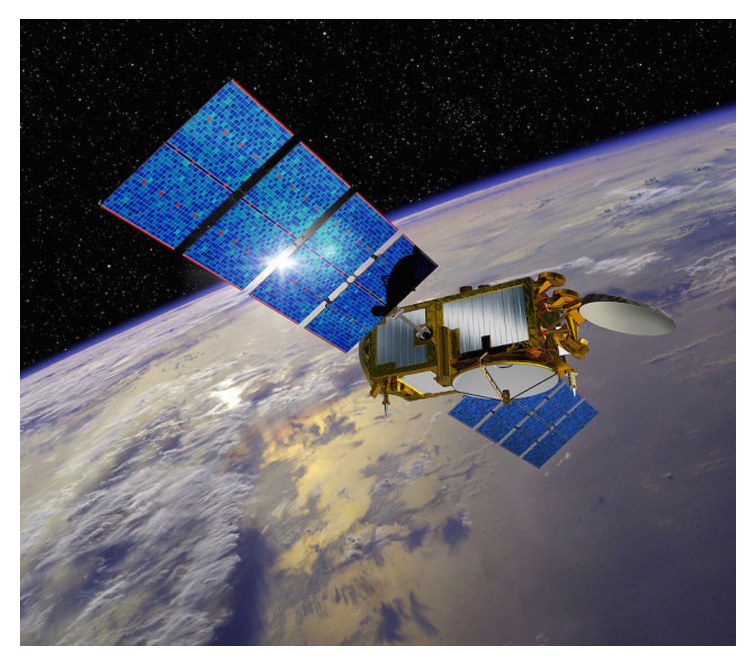
\includegraphics[scale=0.7]{AerospaceApplications/images/satellite_img.png}
    \caption{A satellite on MEO}
\end{figure}

There are many fields in which satellites are used: Earth observation, scientific research, ICT field, other planet observation and so on.\\
Their size is very variable: from few chilos to many tons. During its life a satellite can: reaching a target orbit for a mission for example otherwise a satellite can be exploited to check out some space instrumentation.\\

A satellite can work in one of the three types of orbit. The orbits can be classified in: 
\begin{itemize}
    \itemsep0em
    \item Low Earth Orbit \textbf{(LEO)}: 180-2000 km (above the Earth surface)
    \item Medium Earth Orbit \textbf{(MEO)}: 2000-35000 km
    \item Hight Earth Orbit \textbf{(HEO)}: $\ge$35000 km
\end{itemize}

The topics of this part are divided in this way: 
\begin{enumerate}
    \itemsep0em
    \item \textbf{Attitude dynamics and control}
    \begin{itemize}
        \itemsep0em
        \item rotations, attitude kinematics and dynamics
        \item attitude control
    \end{itemize}
    \item \textbf{Orbital dynamics and control}: 
    \begin{itemize}
        \itemsep0em
        \item orbital dynamics; 
        \item orbital control.
    \end{itemize}
\end{enumerate}

The first part of each chapter will be in order to introduce some theoretical aspect which are fundamental to understand and control a spacecraft. In the part reguarding the \textbf{spacecraft attitude} some results about mathematical tools for rotations are given.


\chapter{Attitude kinematics and dynamics}
\section{Rotations}
\textbf{Rotations} are fundamental to dictate an \textbf{orientation} (often called \textbf{attitude}) to a spacecraft or an aircraft. This is in order to \textit{capture the solar energy}, \textit{make some communication} by using antennas positioned on the Earth surface.\\
In general a spacecraft can be seen as a \textit{rigid body}, whose motion can be described mathematically using a combination of \textbf{rotation} and \textbf{translation}.\\ The objective of this section is to provide a \textbf{set of math tools} in order to sistematically describe this part of the motion. In particular, will be discussed the following techniques:
\begin{enumerate}
    \itemsep0em
    \item Direction cosine matrices (DCM);
    \item Euler angles; 
    \item Angle-axis representation; 
    \item Quaternions; 
\end{enumerate}
All these four techniques are linked in some way, how it will be seen.

\subsection{Reference frames (RF)}
Talking about rotations is fundamental to give the definition of \textbf{reference frame}, from the moment that a rotation is described between \textbf{two different reference frames}. \\

\hspace*{-5mm}
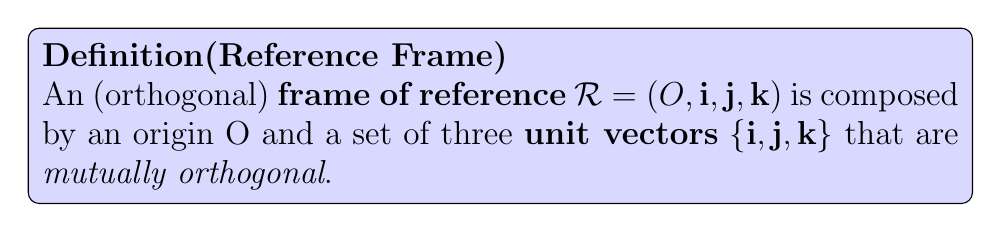
\begin{tikzpicture}
\node [mybox] (box){%
    \begin{minipage}{.96\textwidth}    
        \large{
            \textbf{Definition(Reference Frame)}\\
            An (orthogonal) \textbf{frame of reference} $\mathcal{R}=(O, \mathbf{i,j,k})$ is composed by an origin O and a set of three \textbf{unit vectors} $\{\mathbf{i, j,k}\}$ that are \textit{mutually orthogonal}.
        }
    \end{minipage}
};
\end{tikzpicture}%

\noindent
Given a reference frame $F=\{O, \mathbf{i,j,k}\}$ a vector $\mathbf{r}\in\mathbb{R}^3$ can be expressed in two ways: 
\begin{itemize}
    \itemsep0em
    \item As a \textbf{physical vector}: it is an abstract concept according to which a vector can be expressed as a linear combination of the unit vector, that is: $r=x\mathbf{i}+y\mathbf{j}+z\mathbf{k}$
    \item As a \textbf{coordinate vector}: it is a column vector linked to the specific reference frame $F_\diamond$, that is $$\mathbf{r}=\begin{bmatrix}
        x\\y\\z
    \end{bmatrix}$$ 
\end{itemize}

Then, a generic point/vector in a reference frame has a different representation in another reference frame. The relation beetween two reference frames $F1=\{O,\mathbf{i,j,k}\}$ and $F2=\{O, \mathbf{I,J,K}\}$, introduces to the topic of \textbf{Direction cosine matrices (DCM)}.

\subsection{Direction cosine matrices (DCM)}
In order to introduce a way to link the entities in two reference frames $F1$  and $F2$, let us give a graphical representation of them:

\begin{figure}[h]
    \centering
    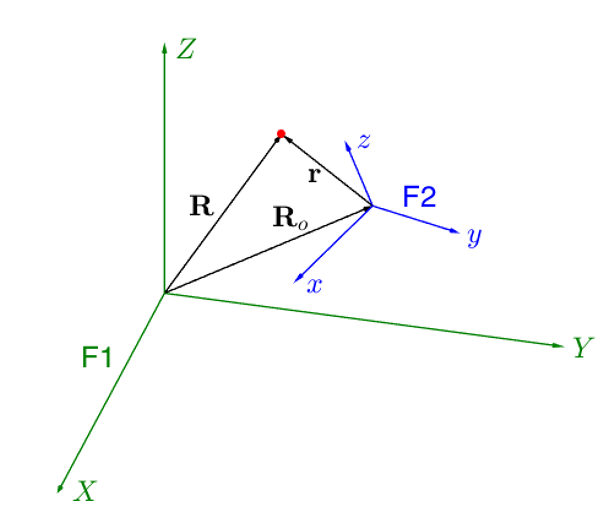
\includegraphics[scale=0.8]{AerospaceApplications/images/RFs.png}
\end{figure}

\noindent
In the above figure the following quantities are shown and a generic particle {\color{red}(in red)} is drawn: 
\begin{equation}
    \begin{aligned}
        &\mathbf{R} = X\mathbf{I} + Y \mathbf{J} + Z \mathbf{K}
        &\text{Position of the particle in F1}\\
        &\mathbf{r} = x \mathbf{i} + y \mathbf{j} + z \mathbf{k}
        &\text{Position of the particle in F2}\\
        &\mathbf{R_O}=X_O \mathbf{I} + Y_O \mathbf{J} + Z_O \mathbf{K}
        &\text{Position in F1 of the O of F2}
    \end{aligned}
\end{equation}
From the geometry follows that $\mathbf{R=R_O+r}$. One wonder at this point \textbf{what is the relation between $X$, $Y$, $Z$ and $x$, $y$, $z$}, using the given former properties we can write:
\begin{equation*}
    \begin{aligned}
        &X = \mathbf{R \cdot I} = \mathbf{(R_O+r) \cdot I} = 
        X_O + x\mathbf{I \cdot i} + y\mathbf{I \cdot j} + 
        z\mathbf{I \cdot k}\\ 
        &Y = \mathbf{R \cdot J} = \mathbf{(R_O+r) \cdot J} = Y_O + x\mathbf{J \cdot i} + y\mathbf{J \cdot j} + 
        z\mathbf{J \cdot k} 
         \\
        &Z = \mathbf{R \cdot K} = \mathbf{(R_O+r) \cdot K} =Z_O + x\mathbf{K \cdot i} + y\mathbf{K \cdot j} + 
        z\mathbf{K \cdot k} \\    
    \end{aligned}
\end{equation*}

Expressed in matrix form:

\begin{equation*}
    \begin{bmatrix}
        X\\Y\\Z
    \end{bmatrix} = 
    \begin{bmatrix}
        X_O\\Y_O\\Z_O
    \end{bmatrix}+
    \begin{bmatrix}
        \mathbf{I \cdot i}&\mathbf{I \cdot j}&\mathbf{I \cdot k}\\
        \mathbf{J \cdot i}&\mathbf{J \cdot j}&\mathbf{J \cdot k}\\
        \mathbf{K \cdot i}&\mathbf{K \cdot j}&\mathbf{K \cdot  k }
    \end{bmatrix}
    \begin{bmatrix}
        x\\y\\z
    \end{bmatrix}, \mathbf{T} \doteq \begin{bmatrix}
        \mathbf{I \cdot i}&\mathbf{I \cdot j}&\mathbf{I \cdot k}\\
        \mathbf{J \cdot i}&\mathbf{J \cdot j}&\mathbf{J \cdot k}\\
        \mathbf{K \cdot i}&\mathbf{K \cdot j}&\mathbf{K \cdot  k }
    \end{bmatrix}
\end{equation*}
The dot products $\mathbf{I \cdot i}$, $\mathbf{I \cdot j}$... represents the \textbf{direction cosine angles} which the axis of one reference frame forms with respect to the other. $\mathbf{T}$ is the \textit{direction cosine matrix}(\textbf{DCM}). 
In literature the DCM can be expressed as:
\begin{equation*}
  \mathbf{T}=\begin{bmatrix}
        T_{11}&T_{12}&T_{13}\\
        T_{21}&T_{22}&T_{23}\\
        T_{31}&T_{32}&T_{33}
    \end{bmatrix}=[T_{ij}]
\end{equation*}
and from the moment that translation and rotation can be studied indipendently, without loss of generality we can assume $\mathbf{R}_O=0$, then the $\mathbf{T}$ becomes a \textbf{transformation matrix} and in particular
\begin{equation*}
    \begin{bmatrix}
        \ X \ \\ \ Y \ \\\ Z \
    \end{bmatrix} = 
    \mathbf{T} 
    \begin{bmatrix}
       \ x \ \\ \ y \ \\ \ z \
    \end{bmatrix}
\end{equation*}
Furthermore, there are \textit{two different interpretation:}
\begin{itemize}
    \itemsep0em
    \item \textbf{Coordinate transformation} from F2 to F1 another term used to indicate this concept is \textit{alias}; 
    \item \textbf{Rotation} of vectors in a given fixed frame, so from F1 to F2, where F2 is the fixed one, another term to indicate this is \textit{alibi}.
\end{itemize}

\subsubsection*{\color{red} Some examples}
Let us consider some examples in 2D, the DCM assumes the form:
\begin{equation*}
    \mathbf{T} = \begin{bmatrix}
        \cos\theta&-\sin\theta\\
        \sin\theta&cos\theta
    \end{bmatrix}
\end{equation*}
From the moment that $z=0$, the third row and the third column of the complete matrix $\mathbf{T}$ disappear.\\

\noindent
{\color{blue} 
\textbf{(\#1) 2D-Coordinate transformation (alias) F2$\to$F1}
}\\
Let us assume that a reference frame F2 is rotated with respect to F1 of an angle $\theta=0.15\pi$, and a particle in F2 is given by
\begin{equation*}
    \mathbf{r} = 0.5\mathbf{i}+0.3\mathbf{j} =
    \begin{bmatrix}
        0.5\\0.3
    \end{bmatrix}
\end{equation*}
The particle coordinates in F1 are obtained through the following transformation
\begin{equation*}
    \begin{bmatrix}
        \ X \ \\ \ Y \
    \end{bmatrix} = \mathbf{Tr} 
\end{equation*}

\begin{figure}[h]
    \centering
    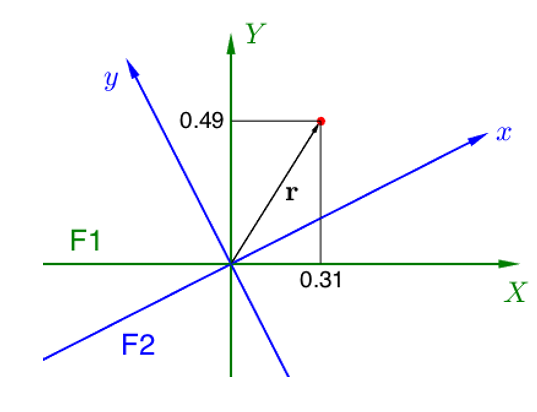
\includegraphics[scale=0.6]{AerospaceApplications/images/coord_transf.png}
    \caption{1st interpretation: Coordinate transformation}
\end{figure}

\noindent
{\color{blue} \textbf{(\#2) 2D-Rotation (alibi) F1$\to$F2}}\\
This time, let us consider a \textbf{vector} $\mathbf{r}$ that in the reference frame F2 is represented by
\begin{equation*}
    \mathbf{r} = \begin{bmatrix}
        \ 0.5 \ \\
        \ 0.3 \
    \end{bmatrix}
\end{equation*}
We can obtain a \textbf{rotated vector} $\mathbf{r}'$ in the same reference frame(fixed) applying the transformation $\mathbf{T}$: 
\begin{equation*}
    \mathbf{r}'=\mathbf{T}\cdot\mathbf{r}
\end{equation*}

\begin{figure}[h]
    \centering
    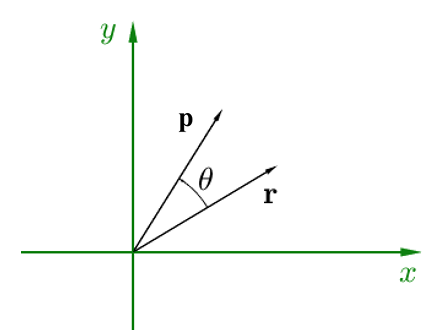
\includegraphics[scale=1]{AerospaceApplications/images/rotation_transf.png}
    \caption{2nd interpretation: rotation in a fixed frame}
\end{figure}

\noindent
{\color{blue} \textbf{(\#3) Rotation of a square in 2D}}
The concept of rotation can be generalized to a 2D-figure like a square for example. A square in 2D can be represented by a matrix $\mathbf{S}\in\mathbb{R}^{2,4}$, which contains by column the (2D)coordinates of the vertices.\\
If we want rotate a square of an angle $\theta$ we can apply the DCM (computed in the angle $\theta$) obtaining a \textbf{rotated square} $\mathbf{S'}$ as follows:
\begin{equation*}
    \mathbf{S'} = \mathbf{T} \cdot \mathbf{S}
\end{equation*}

\begin{figure}[h]
    \centering
    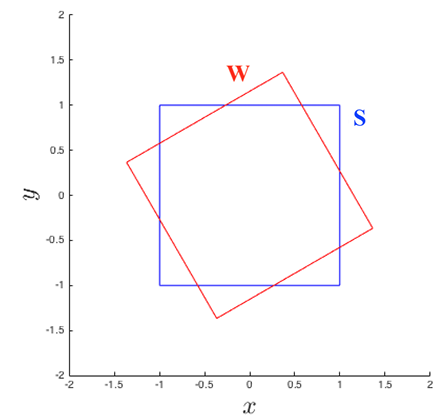
\includegraphics[scale=1]{AerospaceApplications/images/square_rot.png}
    \caption{Rotation of a square}
\end{figure}

\subsection{Euler angles}
In \textbf{three dimensions} we define the \textit{elementary rotation matrices}
\begin{equation*}
    \begin{aligned}
        &\mathbf{T}_1(\phi) = 
        \begin{bmatrix}
            1&0&0\\
            0&\cos\phi&-\sin\phi\\
            0&\sin\phi&cos\phi
        \end{bmatrix} & \text{Rotation about $X$ (or x) of $\phi$ }\\
        &\mathbf{T}_2(\theta) = 
        \begin{bmatrix}
            \cos\theta&0&\sin\theta\\
            0&1&0\\
            -\sin\theta&0&\cos\theta
        \end{bmatrix}  & \text{Rotation about $Y$ (or y) of $\theta$ } \\
        &\mathbf{T}_3(\psi) = \begin{bmatrix}
            \cos\psi&-\sin\psi&0\\
            sin\psi&cos\psi&0\\
            0&0&1
        \end{bmatrix}
        & \text{Rotation about $Z$ (or z) of $\psi$ }\\
    \end{aligned}
\end{equation*}
The interesting thing is that \textbf{any rotation in 3D} can be expressed as a product of $\mathbf{T}_1$, $\mathbf{T}_2$, $\mathbf{T}_3$, moreover the three angles $\phi, \theta, \psi$ are the so-called \textbf{Euler angles}.\\
There are 12 possible combinations of the three elementary matrices of rotations (with non sequentially repeated indexes) they can be divided in \textbf{two groups}: 
\begin{itemize}
    \itemsep0em
    \item[\ding{70}] \textbf{6 Tait-Bryan rotations} the most used are 123 and 321
    \item[\ding{70}] \textbf{6 proper Euler rotations} the most common is 313
\end{itemize}

As they are very used their expression is reported below:

{\color{red}\subsubsection{Tait-Bryan $\mathbf{T}_{123}$}}
\begin{equation*}
    {\large{
        \mathbf{T}_{123}=\begin{bmatrix}
            \cos\theta \cos \psi &
            -cos\theta \sin \psi &
            \sin\theta \\
            \cos\phi\sin\psi + \sin\phi\sin\theta\cos\psi&
            \cos\phi\cos\psi - \sin\phi\sin\theta\sin\psi&
            -\sin\phi\cos\theta\\
            \sin\phi\sin\psi-\cos\phi\sin\theta\cos\psi &
            \sin\phi\cos\psi+\cos\phi\sin\theta\sin\psi &
            \cos\phi\cos\theta
        \end{bmatrix}
    }}
\end{equation*}

{\color{red}\subsubsection{Tait-Bryan $\mathbf{T}_{321}$}}
\begin{equation*}
    {\large{
        \mathbf{T}_{321} = \begin{bmatrix}
            \cos\theta \cos\psi & -\cos\phi \sin\psi +\sin\phi\sin\theta\cos\psi & \sin\phi\sin\psi +\cos\phi \sin\theta \cos\psi\\
            \cos\theta \sin\psi & \cos\phi \cos\psi +\sin\phi\sin\theta\sin\psi & -\sin\phi\cos\psi +\cos\phi \sin\theta \sin\psi\\
            -\sin\theta & \sin\phi\cos\theta&\cos\phi\cos\theta
        \end{bmatrix}
    }}
\end{equation*}


{\color{red}\subsubsection{Proper Euler $\mathbf{T}_{313}$}}
\begin{equation*}
    {\large{
        \mathbf{T}_{313} = \begin{bmatrix}
            \cos\phi \cos\psi - \sin\phi \cos\theta \sin\psi & -\cos\phi \sin\psi -\sin\phi \cos\theta \cos\psi & \sin\phi \sin\theta\\
            \sin\phi \cos\psi + \cos\phi \cos\theta \sin\psi & -sin\phi \sin\psi + \cos\phi \cos\theta \cos\psi & -cos\phi \sin\theta\\
            \sin\theta \sin\psi & \sin\theta \cos\psi & \cos\theta 
    \end{bmatrix}
    }} 
\end{equation*}

\subsection{Rotation matrices general properties}
The following are \textbf{general properties} related to the rotation matrices. \textbf{Notation}: we indicate with $\mathbf{T}_{\diamond}$ any composition of the elementary rotation matrices (with non-sequentially repeated elements).\\
Matrices $\mathbf{T}_{\diamond}$ have the following properties:
\begin{itemize}
    \itemsep0em
    \item[\ding{70}] They are \textbf{linear transformations}, from the product of linear matrices;
    \item[\ding{70}] They are \textbf{orthogonal matrices}, that is matrices whose columns are composed of real entries and are \textbf{orthonormal}. The most important property is: 
    $$\mathbf{T}_{\diamond}^T=\mathbf{T}_{\diamond}^{-1}, \quad 
    \mathbf{T}_{\diamond}^{T}\mathbf{T}_{\diamond}=\mathbf{T}_{\diamond}\mathbf{T}_{\diamond}^T=\mathbf{I}$$
    \textbf{orthogonal transformations} preserve:
    \begin{itemize}
        \itemsep0em
        \item the \textbf{length} of the vectors;
        \item the \textbf{angles} between the vectors;
    \end{itemize}
    $$\text{length} + \text{angles} \Longrightarrow \textbf{shape preserved}$$
    \item[\ding{70}] Their \textbf{eigenvalues} are always $\{1, \pm e^{j\beta}\}$, their \textbf{determinant} always equal to 1;
\end{itemize} 

{\color{blue}\subsubsection{Singularities, Gimbal lock}}
For certain values of $\theta$ some matrices can present some \textbf{singularities}, for example the matrix $\mathbf{T}_{123}$. For example if $\theta=\frac{\pi}{2}$ only the sum $(\psi+\phi)$ can be determined and this results in a \textbf{loss of degree of freedom} $\Longrightarrow$ this phenomenon is also known as \textbf{gimbal lock} and affect all the \textit{gyroscopes} in which two out of three axes are aligned and this results in a loss of a degree of freedom, in \textit{normal situations} the three axis, instead, can rotate indipendently.
In order to overcome this problem, we use non minimal representation in which instead of only three variables, are used \textbf{four variables}.\\
More in general, \textbf{there is always a gimbal lock} when: 
\begin{itemize}
    \itemsep0em
    \item[\ding{70}] In the \textbf{Tait-Bryan rotations}, $\cos\theta=0$;
    \item[\ding{70}] In the \textbf{Proper Euler rotations}, when occurs that $\sin\theta=0$   
\end{itemize}
This singularities cause problems in the \textit{kinematic equation} like divergent behaviour, this is the reason why alternative method to manage these situations are required.

\begin{figure}[h]  
    \centering
    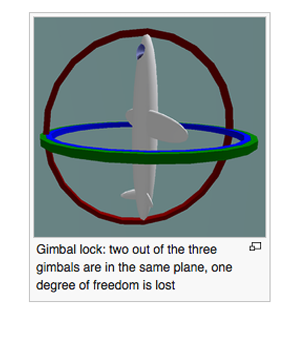
\includegraphics[scale=1.3]{AerospaceApplications/images/gimbal_lock.png}
    \caption{Gimbal lock example}
\end{figure}

\subsection{Euler's rotation theorem}
The following theorem is very important because it introduces an alternative way to describe rotations: \\

\hspace*{-5mm}
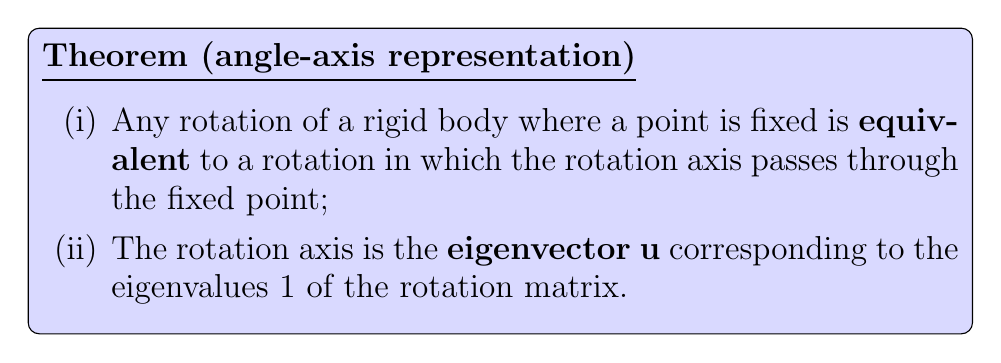
\begin{tikzpicture}
\node [mybox] (box){%
    \begin{minipage}{.96\textwidth}     %Larghezza del box
        \large{
            \textbf{\underline{Theorem (angle-axis representation)}}
            \begin{itemize}
                \itemsep0em
                \item[(i)] Any rotation of a rigid body where a point is fixed is \textbf{equivalent} to a rotation in which the rotation axis passes through the fixed point; 
                \item[(ii)] The rotation axis is the \textbf{eigenvector} $\mathbf{u}$ corresponding to the eigenvalues 1 of the rotation matrix. 
                \vspace{0.2cm}
            \end{itemize} 
        }
    \end{minipage}
};
\end{tikzpicture}%

\vspace{0.5cm}
\noindent
\textbf{\textit{Proof}}\\
The rotation matrix $\mathbf{T}_{\diamond}$ has a unitary eigenvalue, it holds (from the definition) that: $\mathbf{T}_{\diamond}\mathbf{u}=\mathbf{u}$, so the rotation does not change the direction $\mathbf{u}$, which is the rotation axis. $_\square$\\

From this theorem, follows that \textit{any rotation} can be described by using two quantities involving four variables: 
\begin{itemize}
    \itemsep0em
    \item[\ding{70}] An angle $\beta$ (1 variable)
    \item[\ding{70}] A rotation axis $\mathbf{u}$ (3 variables)
\end{itemize}
\huge{
\begin{equation*}
    \mathbf{T} \equiv \mathbf{T}(\beta, \mathbf{u})
\end{equation*}}





\subsection{Quaternions}

\subsection{Change of representation}


\chapter{Attitude kinematics and dynamics}
\chapter{Attitude control}
\chapter{Orbital dynamics}
\chapter{Orbital control}

\end{document}

%nel main prima di \begin{document}




